\newif\ifuseudlogo
% uncomment the following line if you want the UD logo in the title page
\useudlogotrue

\documentclass[11pt,ms]{uddissert2019}
\usepackage{uddissert2019-mods}
\usepackage{graphicx}
\usepackage{appendix}
\usepackage{xcolor} % for coloring text

\usepackage{subfig}
\usepackage{epsfig}
\usepackage{amsmath}

\graphicspath{
	{./figures/introduction/}
	{./figures/experimental_setup/}
	{./figures/dataset/}
	{./figures/grid_search_results/}
	{./figures/test_results/}}

\begin{document}

\pagestyle{intropage}

\authorLastFirstMiddle{Grose}{Mitchell Gene}
\firsttitle{FORECASTING ATMOSPHERIC TURBULENCE CONDITIONS FROM PRIOR ENVIRONMENTAL PARAMETERS WITH ARTIFICIAL NEURAL NETWORKS: AN ENSEMBLE STUDY}
\title{FORECASTING ATMOSPHERIC TURBULENCE CONDITIONS FROM PRIOR ENVIRONMENTAL PARAMETERS WITH ARTIFICIAL NEURAL NETWORKS: AN ENSEMBLE STUDY}

\graduationyear{2021}%
\graduationmonth{May}%
\school{The School of Engineering}%
\dept{Engineering}

\advisorFirstLast{Eric J. Balster}{, Ph.D.}{Advisory Committee
Chairman}{Associate Professor and Chair}{Electrical and Computer Engineering} %
\Membera{Member A.}{, Ph.D.}{Committee Member}{Faculty A. Title}{Faculty A department}%
\Memberb{Member B.}{, Ph.D.}{Committee Member}{Faculty B. Title}{Faculty B department}%
\Memberc{Member C.}{, Ph.D.}{Committee Member}{Faculty C. Title}{Faculty C department}%
%\Memberd{Member D.}{, Ph.D.}{Committee Member}{Faculty D. Title}{Faculty D department}%

\AssocDean{Robert J. Wilkens, Ph.D., P.E.}{Associate Dean for Research and Innovation Professor}{School of Engineering}%
\Dean{Eddy M. Rojas, Ph.D., M.A., P.E.}{Dean, School of Engineering}%

\makethesistitle

\disscopyright
% use above to include a copyright page

\abstract
Optical (atmospheric) turbulence ($C_{n}^{2}$) is a highly stochastic process that can apply many adverse effects on imaging and laser propagation systems. Modeling atmospheric turbulence conditions has been proposed by physics-based models but they are unable to capture the many cases. Recently, machine learning surrogate models have been used to learn the relationship between local environmental (weather) and turbulence conditions. These models predict a turbulence strength at time $t$ from weather at time $t$. This thesis proposes a technique to forecast four hours of future turbulence conditions at 30-minute intervals from prior environmental parameters using artificial neural networks. First, local weather and turbulence measurements are formatted to pairs of input sequence and output forecast. Next, a grid search is performed to find the best combination of model architecture and training parameters. The architectures investigated are the Multilayer Perceptron (MLP) and three variants of the Recurrent Neural Network (RNN). Finally, the selected model is applied to the test dataset and analyzed. It is shown that the model has generally learned the relationship between prior environmental and future turbulence conditions.

\dedication{For name of person(s) to whom you are dedicating your thesis}

\acknowledgments
\begin{enumerate}
	\item Professor Edward Watson - Advisor
	\item Colleagues at MZA Associates Corporation
	\begin{enumerate}
		\item Dr. Matthew Whiteley
		\item Dr. Jason Schmidt
		\item Dr. Yakov Diskin
	\end{enumerate}
	\item Researchers at OSU
	\begin{enumerate}
		\item Professor David Bromwich (OSU) - Undergraduate Research Professor
		\item Dr. Sheng-Hung Wang (OSU) - Undergraduate Research Tutor
	\end{enumerate}
	\item Professor Shawn Ryan (CSU) - Undergraduate Math Professor
	\item Family (particularly Mom and Dad) and friends
\end{enumerate}




\tableofcontents


\listoffigures
\listoftables

\pagestyle{plain}
%Remember to put all chapter titles in CAPS
\addtocontents{toc}{\protect\setChapterprefix{CHAPTER }} % CDM Establish CHAPTER label in table of contents

\chapter{Introduction Problem Statement; Literature Review}
\label{ch1}

\section{Problem Statement}
\subsection{This effort performs an ensemble study of ML architectures/parameters to best forecast 4 hours of turbulence conditions from prior measurements.}

\subsection{What is turbulence ($C_{n}^{2}$)? Why is it important to measure/model?}
\begin{figure}[h!]
	\centering
	\subfloat[Low-strength ($C_{n}^{2}$)\label{fig:first_frames_a}]{
		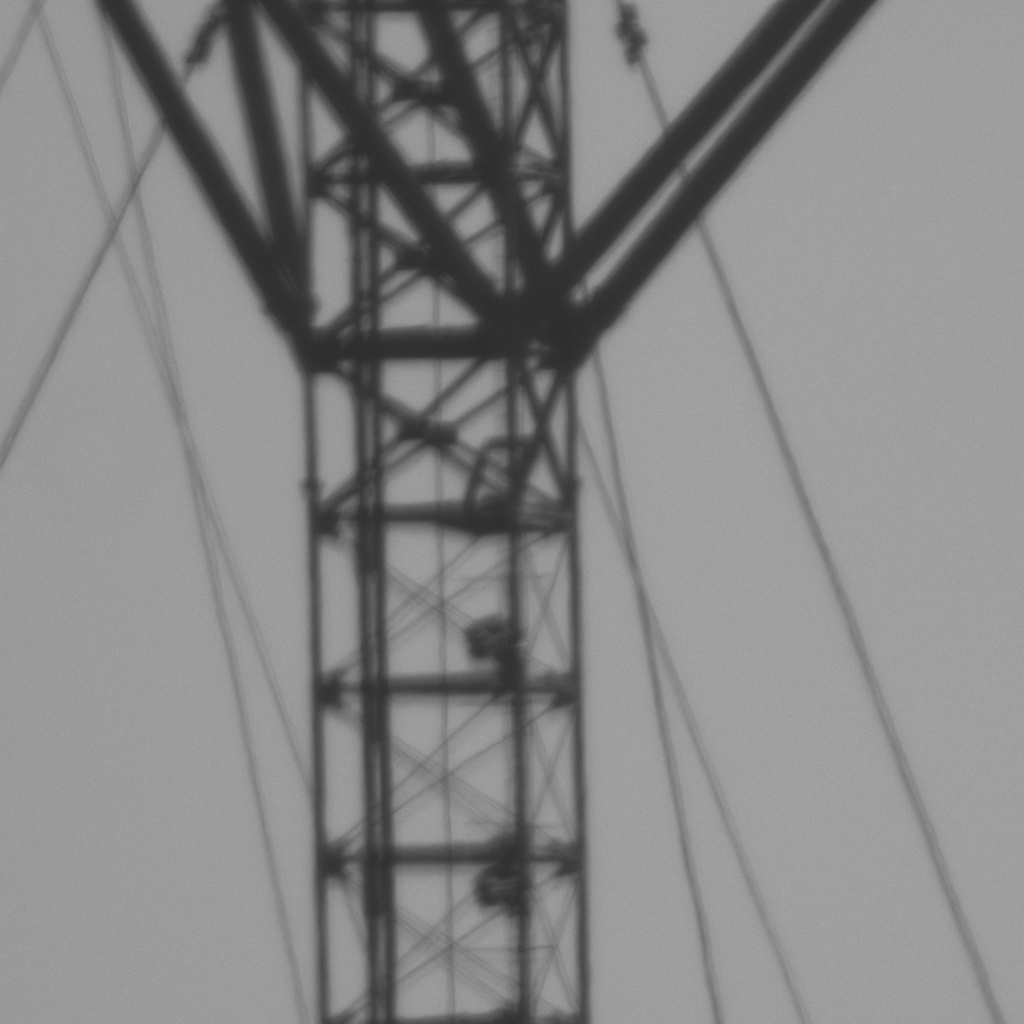
\includegraphics[width=0.49\textwidth]
		{FirstFrame_LowTurb.jpg}
	}
	\subfloat[High-strength ($C_{n}^{2}$)\label{fig:first_frames_b}]{
		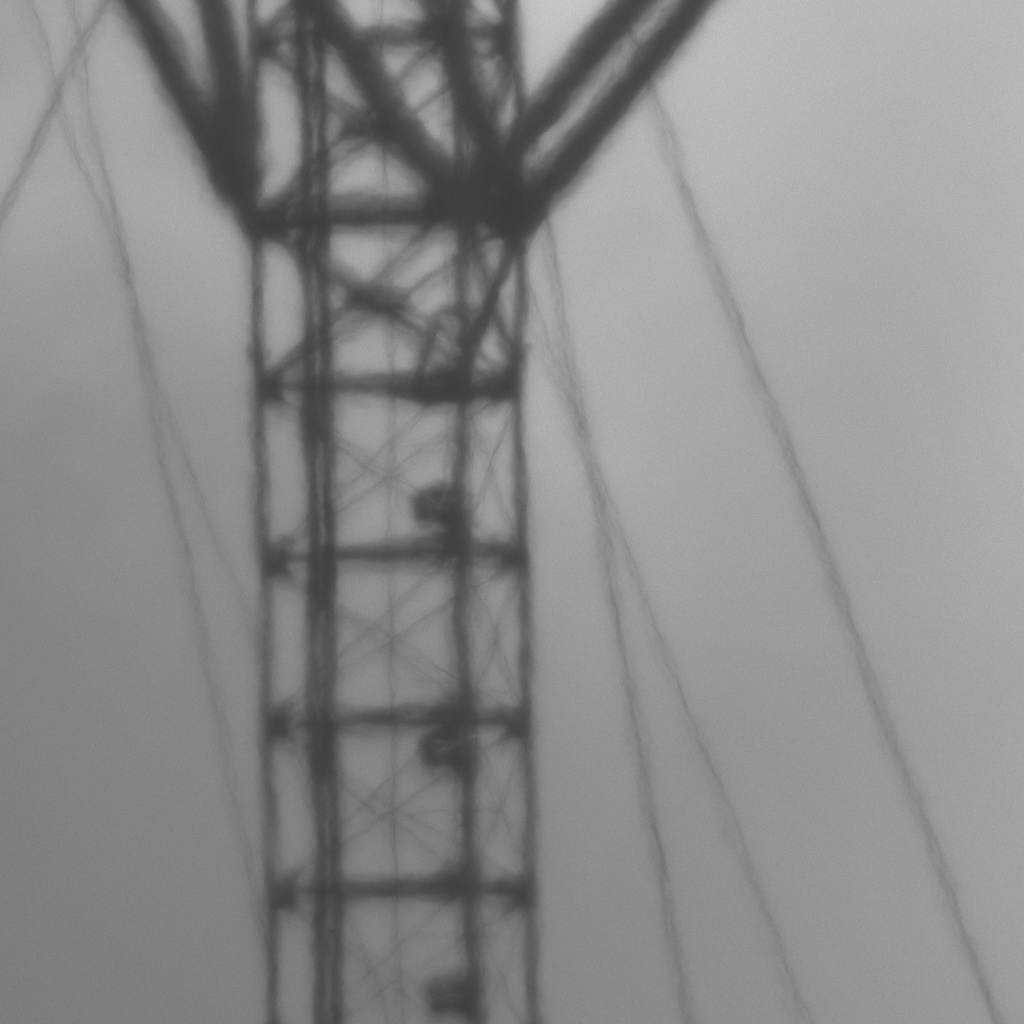
\includegraphics[width=0.49\textwidth]
		{FirstFrame_HighTurb.jpg}
	}
	\hfill
	\caption{Effect of low-strength and high-strength $C_{n}^{2}$ conditions.}
	\label{fig:first_frames}
\end{figure}

\subsection{Review the fundamentals of machine learning.}
Optimization algorithm!
\begin{figure}[h!]
	\centering
	\subfloat[Training\label{fig:simple_model_training_testing_a}]{
		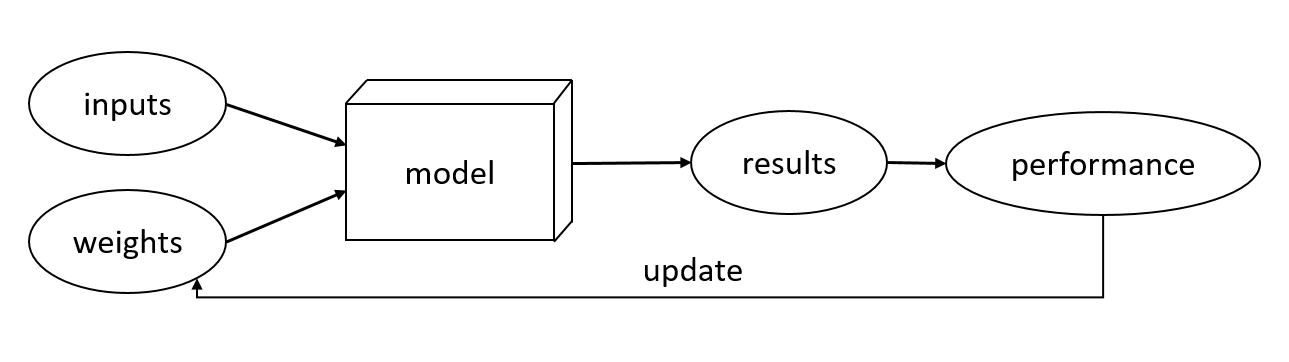
\includegraphics[width=0.99\textwidth]
		{training_process.png}
	}
	\hfill
	\subfloat[Testing\label{fig:simple_model_training_testing_b}]{
		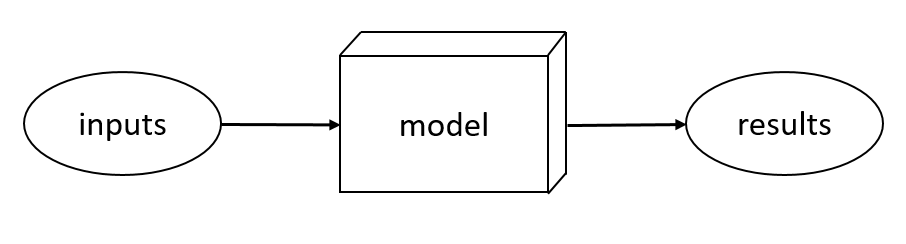
\includegraphics[width=0.99\textwidth]
		{testing_process.png}
	}
	\hfill
	\caption{Simple example of machine learning model training and testing.}
	\label{fig:simple_model_training_testing}
\end{figure}

\section{Literature Review}
\subsection{State of Turbulence $C_{n}^{2}$ Modeling}
\subsubsection{Physical Models}
\subsubsection{ML Models}
Recently published literature predicts $C_{n}^{2}$ conditions at time \textit{t} given weather inputs at time \textit{t}.
\subsection{General information about MLP/RNN architectures here? Does the in-depth review of the architectures go here?}
\chapter{Machine Learning Modeling Review}
\label{ch2}
PyTorch reference \cite{NEURIPS2019_9015}.
Colah's blog reference \cite{olah}.
\section{Fundamentals of Training and Testing}
\begin{figure}[h!]
	\centering
		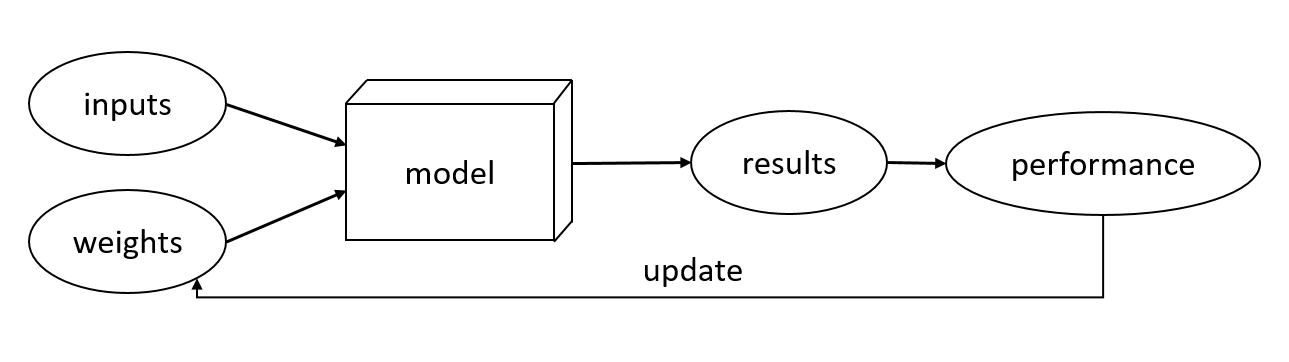
\includegraphics[width=0.99\textwidth]
		{training_process.png}
		\hfill
		\caption{Simple example of machine learning model training .}
		\label{fig:simple_model_training}
\end{figure}

\begin{figure}[h!]
	\centering
	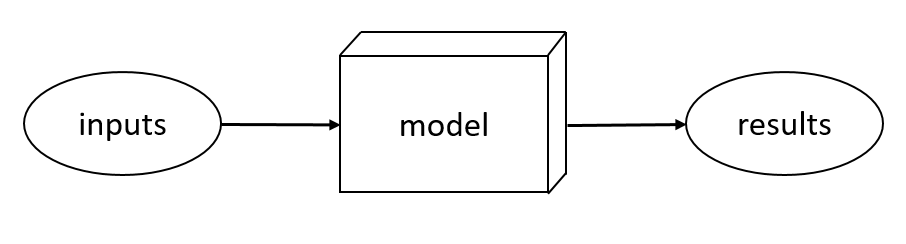
\includegraphics[width=0.99\textwidth]
	{testing_process.png}
	\hfill
	\caption{Simple example of machine learning model testing.}
	\label{fig:simple_model_testing}
\end{figure}

\section{MLP and RNN Architectures}
\subsection{MLP}
\begin{figure}[h!]
	\centering
	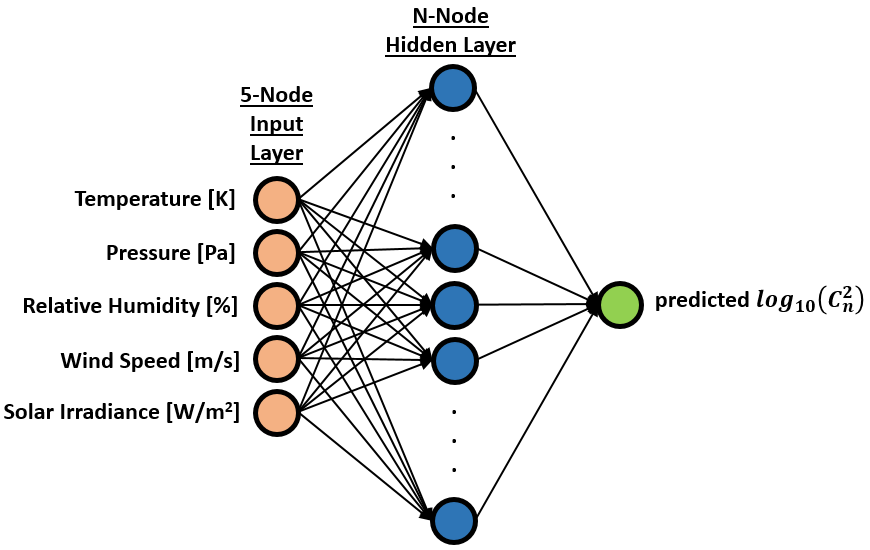
\includegraphics[width=0.99\textwidth]
	{architecture_MLP_simple.png}
	\hfill
	\caption{Simple MLP (multi-layer perceptron) to predict $log_{10}(C_{n}^{2})$ from weather inputs.}
	\label{fig:architecture_MLP_simple}
\end{figure}

\begin{figure}[h!]
	\centering
	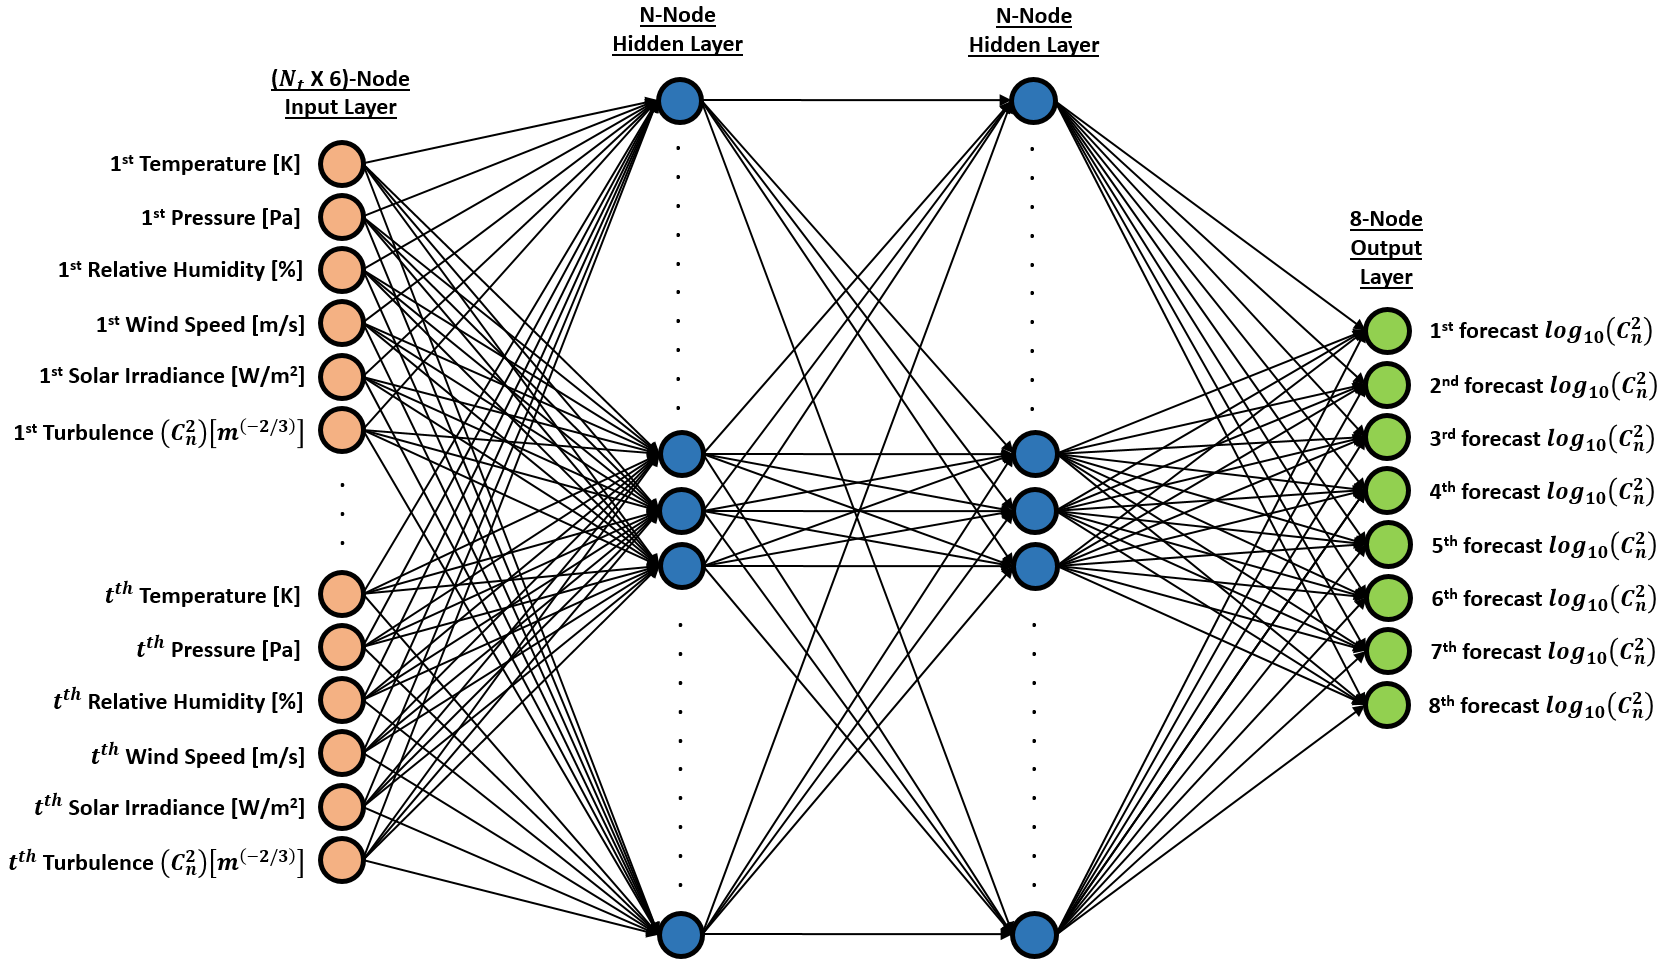
\includegraphics[width=0.99\textwidth]
	{achitecture_MLP_forecast.png}
	\hfill
	\caption{MLP to forecast eight time steps of $log_{10}(C_{n}^{2})$ from multiple time steps of weather inputs.}
	\label{fig:achitecture_MLP_forecast}
\end{figure}

\begin{equation} \label{eq:MLP}
	y = \sigma \left(xW + b\right)
\end{equation}
where $x$ is the input, $W$ is the learnable weights and $b$ is the learnable bias.

\clearpage

\subsection{RNN}
\begin{figure}[h!]
	\centering
	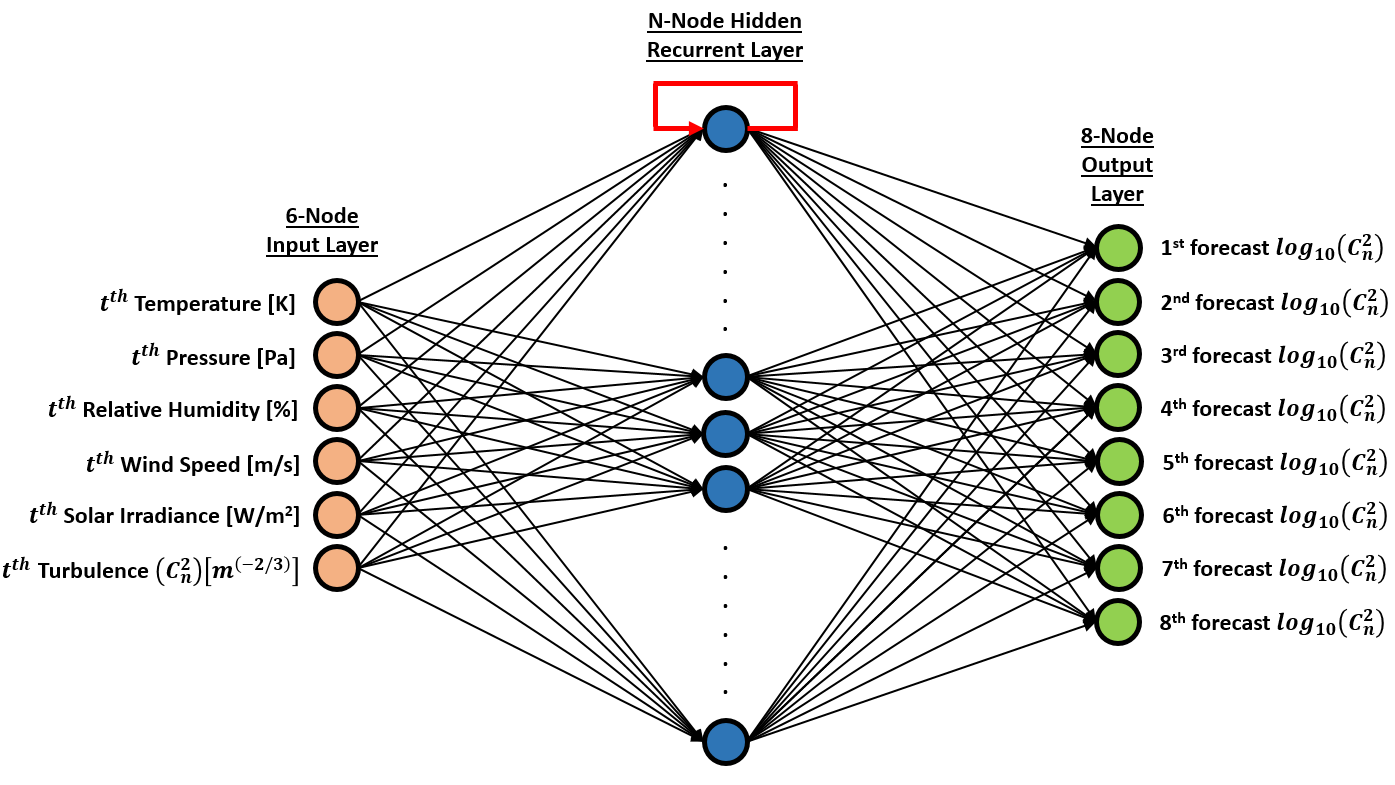
\includegraphics[width=0.99\textwidth]
	{architecture_RNN_single_layer.png}
	\hfill
	\caption{Single-layer RNN architecture to forecast eight time steps of $log_{10}(C_{n}^{2})$ from multiple time steps of weather inputs processed by the recurrent layer.}
	\label{fig:architecture_RNN_single_layer}
\end{figure}

\begin{figure}[h!]
	\centering
	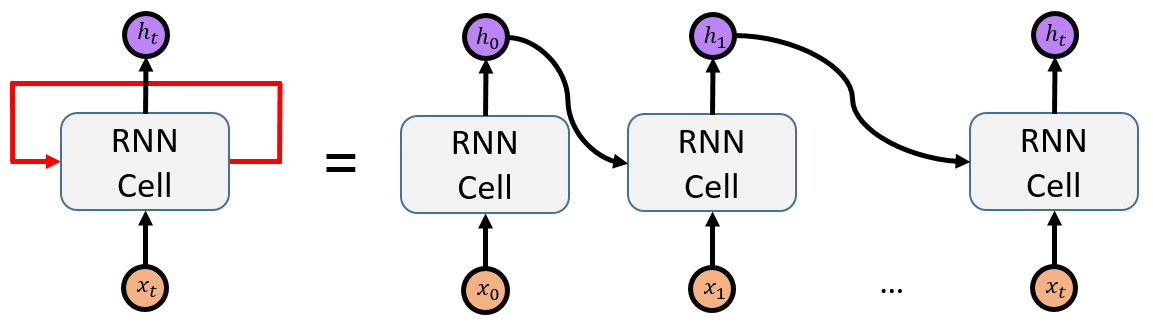
\includegraphics[width=0.99\textwidth]
	{architecture_RNN_single_layer_unrolled.png}
	\hfill
	\caption{Unrolled single-layer RNN}
	\label{fig:architecture_RNN_single_layer_unrolled}
\end{figure}

\begin{figure}[h!]
	\centering
	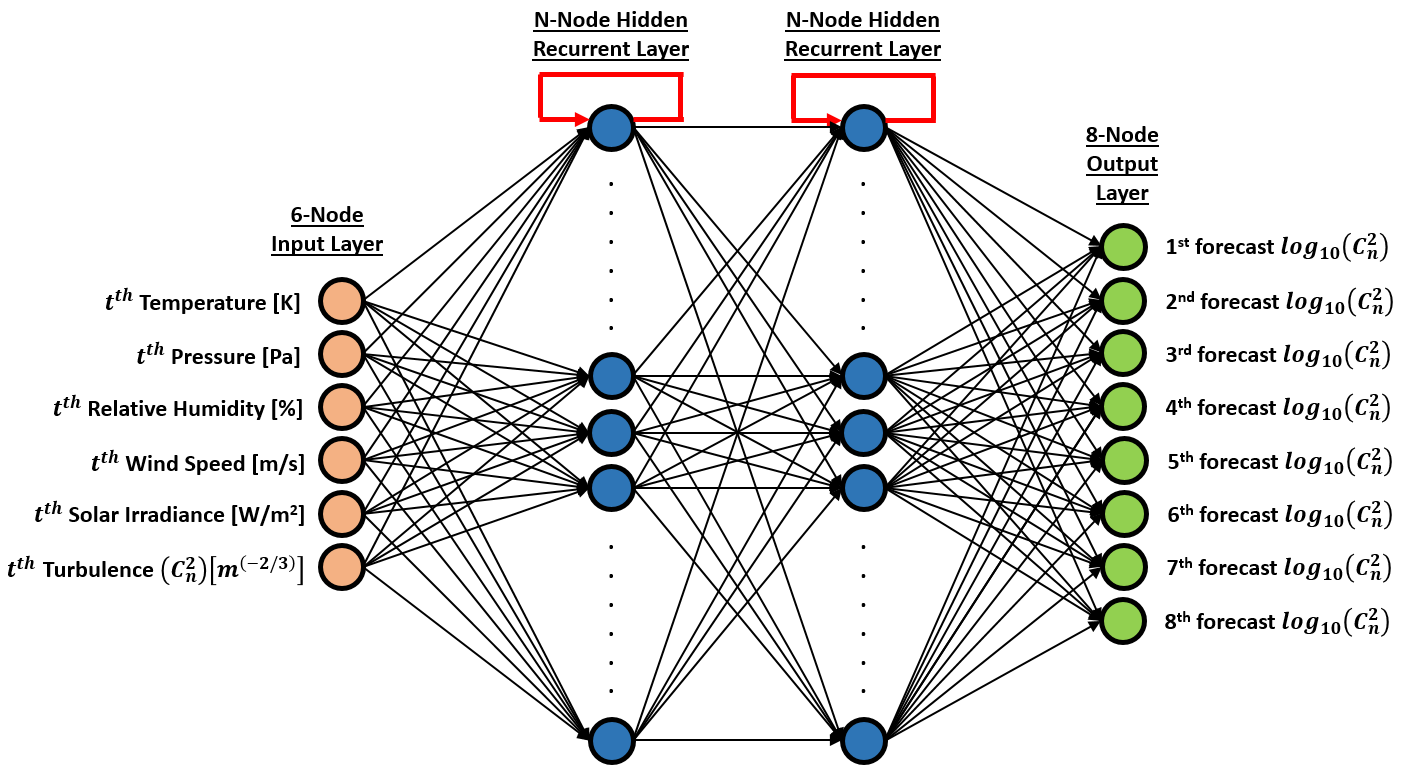
\includegraphics[width=0.99\textwidth]
	{architecture_RNN_multi_layer.png}
	\hfill
	\caption{Multi-layer RNN architecture to forecast eight time steps of $log_{10}(C_{n}^{2})$ from multiple time steps of weather inputs processed by the recurrent layers.}
	\label{fig:architecture_RNN_multi_layer}
\end{figure}

\begin{figure}[h!]
	\centering
	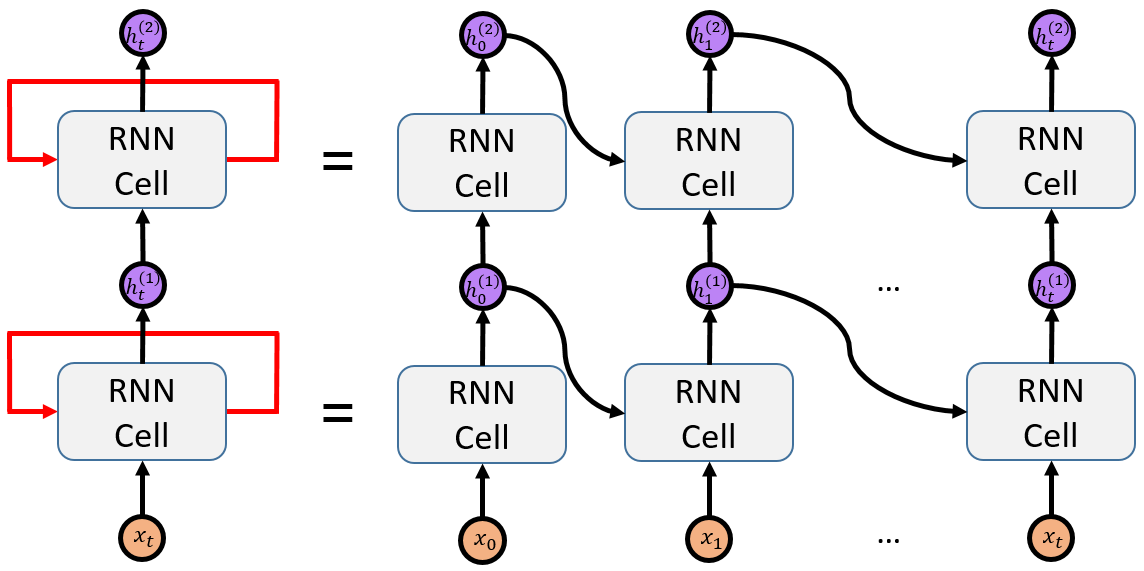
\includegraphics[width=0.99\textwidth]
	{architecture_RNN_multi_layer_unrolled.png}
	\hfill
	\caption{Unrolled multi-layer RNN}
	\label{fig:architecture_RNN_multi_layer_unrolled}
\end{figure}
A recurrent neural network (RNN) is a neural network that operates on a variable-length sequence. The RNN processes the sequence input with a hidden state $h$ whose activation (value) at each time $t$ is dependent on the activation of the previous time. At each time step $t$ the hidden state $h_{t}$ of the RNN is updated by
\begin{equation} \label{eq:RNN}
	h_{t} = \tanh\left(W_{ih}x_{t} + b_{ih} + W_{hh}h_{\left(t-1\right)} + b_{hh}\right)
\end{equation}
where $x_{t}$ is the input at time $t$, $h_{\left(t-1\right)}$ is the hidden state of the previous layer at time $t-1$ or the initial state at time 0 (zero), $W_{ih}$ is the learnable input-hidden weights, $b_{ih}$ is the learnable input-hidden bias, $W_{hh}$ is the learnable hidden-hidden weights, and $b_{hh}$ is the learnable hidden-hidden bias \cite{NEURIPS2019_9015}.

\begin{figure}[h!]
	\centering
	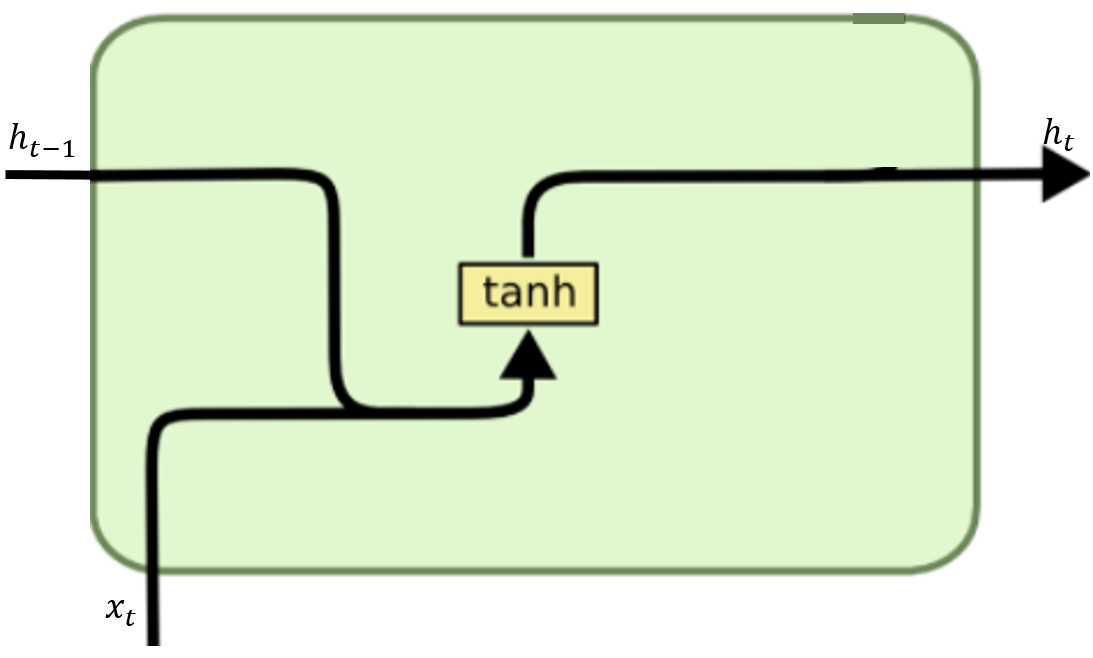
\includegraphics[width=0.7\textwidth]
	{cell_RNN.png}
	\hfill
	\caption{Simple RNN cell}
	\label{fig:cell_RNN}
\end{figure}

\clearpage

\subsection{LSTM}
For each element in the input sequence, each layer computes the following function:
\begin{align}
	i_{t} &= \sigma\left(W_{ii}x_{t} + b_{ii} + W_{hi}h_{\left(t-1\right)} + b_{hi}\right) \label{eq:LSTM1} \\
	f_{t} &= \sigma\left(W_{if}x_{t} + b_{if} + W_{hf}h_{\left(t-1\right)} + b_{hf}\right) \label{eq:LSTM2} \\
	g_{t} &= \tanh\left(W_{ig}x_{t} + b_{ig} + W_{hg}h_{\left(t-1\right)} + b_{hg}\right) \label{eq:LSTM3} \\
	o_{t} &= \sigma\left(W_{io}x_{t} + b_{io} + W_{ho}h_{\left(t-1\right)} + b_{ho}\right) \label{eq:LSTM4} \\
	c_{t} &= f_{t} \odot c_{\left(t-1\right)} + i_{t} \odot g_{t} \label{eq:LSTM5} \\
	h_{t} &= o_{t} \odot \tanh\left(c_{t}\right) \label{eq:LSTM6}
\end{align}
where $h_{t}$ is the hidden state at time $t$, $c_{t}$ is the cell state at time $t$, $x_{t}$ is the input at time $t$, $h_{\left(t-1\right)}$ is the hidden state of the layer at time $t-1$ or the initial state at time 0 (zero), and $i_{t}$, $f_{t}$, $g_{t}$, and $o_{t}$ are the input, forget, cell, and output gates, respectively. $W_{ii}$, $W_{if}$, $W_{ig}$, and $W_{io}$ are the learnable input-hidden weights for the input, forget, cell, and output gates. $\sigma$ is the sigmoid function, and $\odot$ is the Hadamard (element-wise) product \cite{NEURIPS2019_9015}.

\begin{figure}[h!]
	\centering
	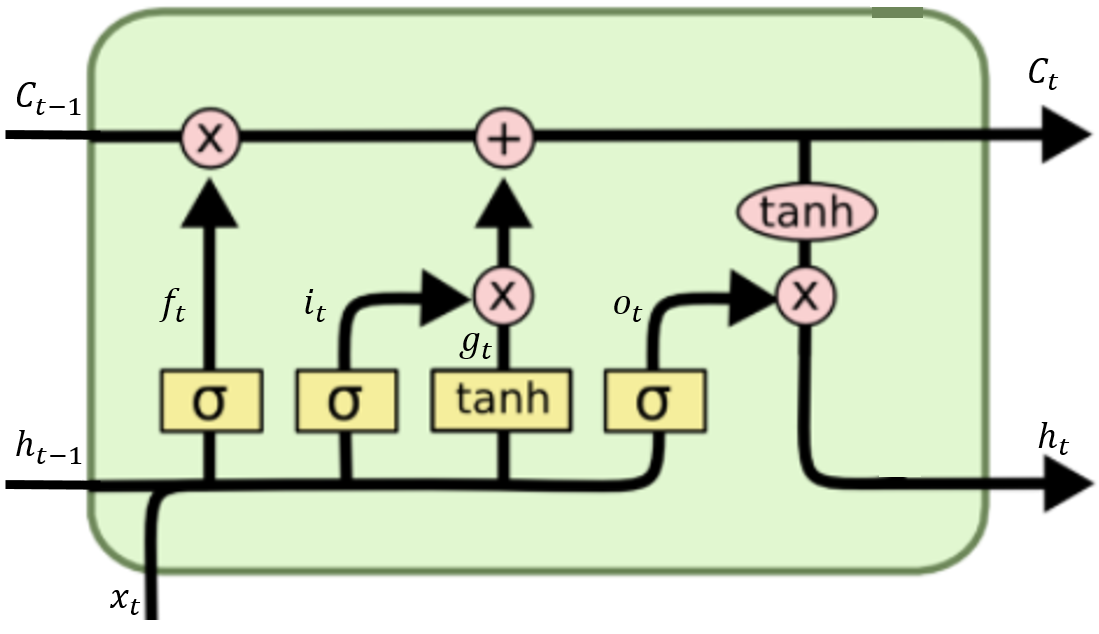
\includegraphics[width=0.7\textwidth]
	{cell_LSTM.png}
	\hfill
	\caption{LSTM-RNN cell}
	\label{fig:cell_LSTM}
\end{figure}

\subsection{GRU}
For each element in the input sequence, each layer computes the following function:
\begin{align}
	r_{t} &= \sigma\left(W_{ir}x_{t} + b_{ir} + W_{hr}h_{\left(t-1\right)} + b_{hr}\right) \label{eq:GRU1} \\
	z_{t} &= \sigma\left(W_{iz}x_{t} + b_{iz} + W_{hz}h_{\left(t-1\right)} + b_{hz}\right) \label{eq:GRU2} \\
	n_{t} &= \tanh\left(W_{in}x_{t} + b_{in} + r_{t} \odot \left(W_{hn}h_{\left(t-1\right)} b_{hn}\right)\right) \label{eq:GRU3} \\
	h_{t} &= \left(1 - z_{t}\right) \odot n_{t} + z_{t} \odot h_{\left(t-1\right)} \label{eq:GRU4}
\end{align}
where $h_{t}$ is the hidden state at time $t$, $x_{t}$ is the input at time $t$, $h_{\left(t-1\right)}$ is the hidden state of the layer at time $t-1$ or the initial hidden state at time 0 (zero), and $r_{t}$, $z_{t}$, and $n_{t}$ are the reset, update, and new gates, respectively. $W_{ir}$, $W_{iz}$ and $W_{in}$ are the learnable input-hidden weights for the reset, update, and new gates, respectively, and are of shape $numlayers \times 3hiddensize \times inputsize$. $W_{hr}$, $W_{hz}$ and $W_{hn}$ are the learnable hidden-hidden weights for the reset, update, and new gates, respectively, and are of shape $numlayers \times 3hiddensize \times inputsize$. $b_{ir}$, $b_{iz}$, and $b_{in}$ are the learnable input-hidden biases of the reset, update, and new gates, respectively. $b_{hr}$, $b_{hz}$, and $b_{hn}$ are the learnable hidden-hidden biases of the reset, update, and new gates, respectively. $\sigma$ is the sigmoid function, and $\odot$ is the Hadamard (element-wise) product \cite{NEURIPS2019_9015}. 

\begin{figure}[h!]
	\centering
	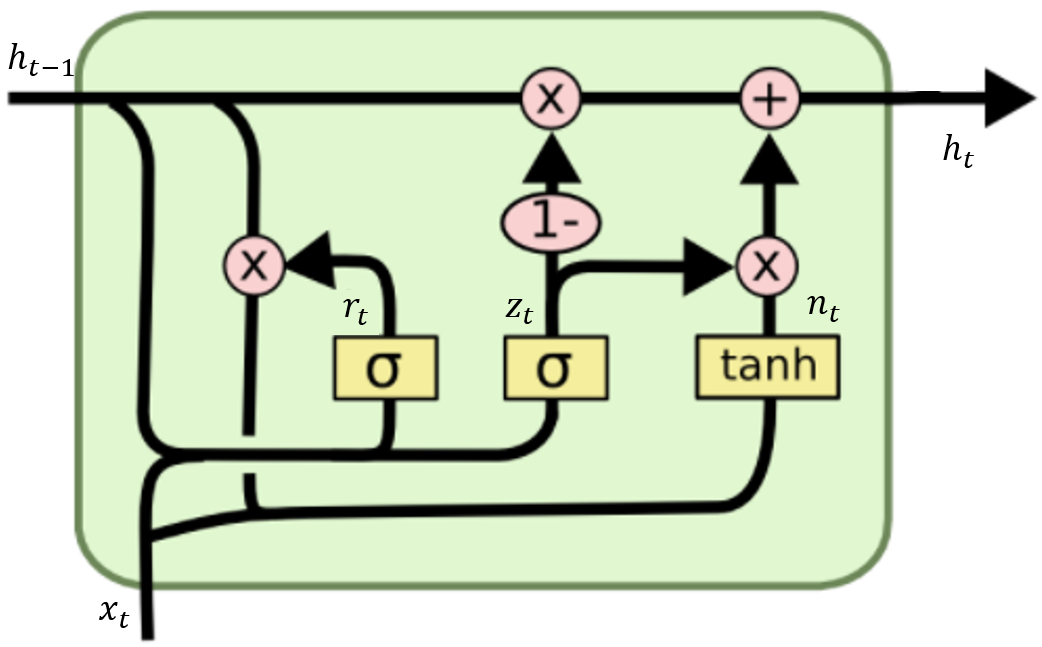
\includegraphics[width=0.7\textwidth]
	{cell_GRU.png}
	\hfill
	\caption{GRU-RNN cell}
	\label{fig:cell_GRU}
\end{figure}

\section{Optimization and Loss Function}
Neural networks are a collection of nested functions that are executed on some input data. These functions are defined by \emph{parameters} (weights and biases). The training of a neural network is the process of updating the parameters to reduce the loss between network outputs and truth values. Training happens in two steps. The first step is forward propagation in which the network makes a prediction by passing input values through its functions (applying the weights and biases). The second step is backward propagation where the network adjusts its parameters proportionate to the error in its prediction. The network does this by moving backwards through the network from the output, collecting the derivatives of the error with respect to the parameters of the functions and optimizing the parameters using gradient descent. The derivatives of the error with respect to the parameters are called gradients. PyTorch's automatic differentiation engine \textit{autograd} handles this entire process \cite{NEURIPS2019_9015}.

Follow 3Blue1Brown video but with my own images and notations. Start with a 1x1 then move to a 2x2 network?
``These chain rule expressions give you the derivatives that determine each component in the gradient that helps minimize the loss of the network by repeatedly stepping downhill." - 3Blue1Brown

\section{Chapter Summary?}
\chapter{Dataset}
\label{ch3}


\section{Weather Sequences}
Temporal sequence plots presented in Figure \ref{fig:sequence_temporal}.
\begin{figure}[p!]
	\centering
	\subfloat[Temperature (K)\label{fig:sequence_temporal_a}]{
		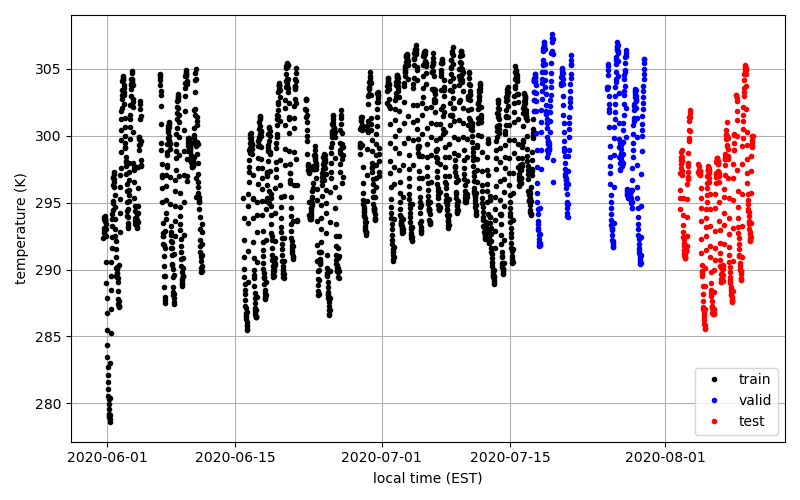
\includegraphics[width=0.49\textwidth]{temporal_sequence_temp.png}
	}
	\subfloat[Pressure (Pa)\label{fig:sequence_temporal_b}]{
		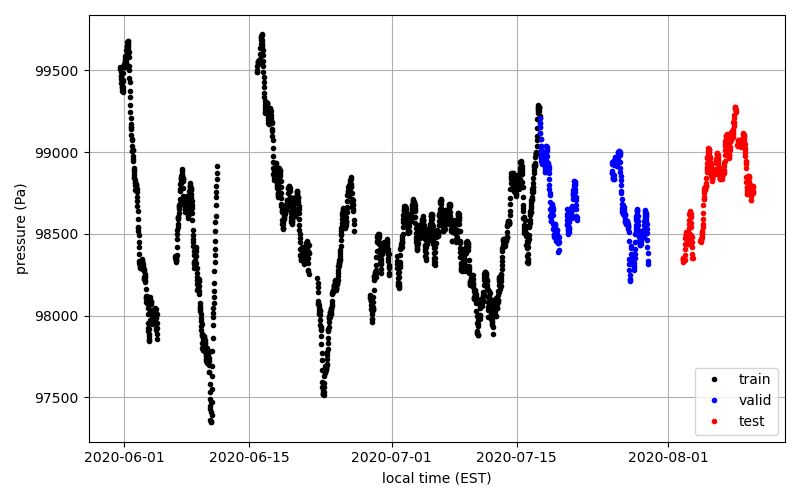
\includegraphics[width=0.49\textwidth]{temporal_sequence_press.png}
	}
	\hfill
	\subfloat[Relative Humidity (\%)\label{fig:sequence_temporal_c}]{
		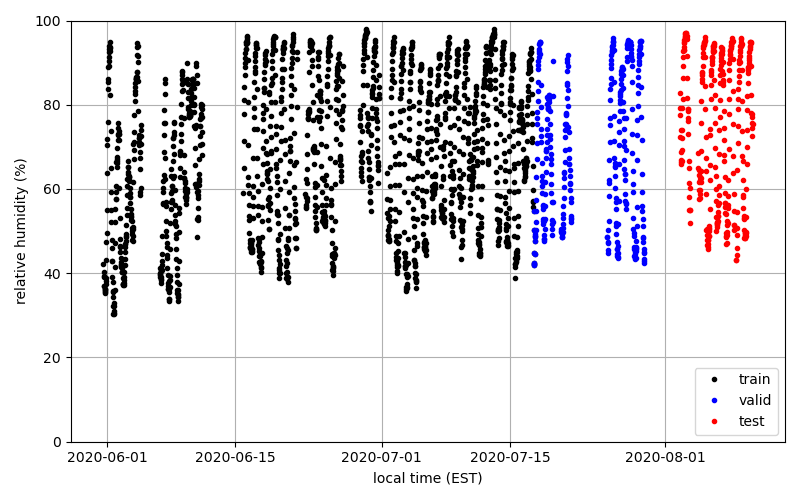
\includegraphics[width=0.49\textwidth]{temporal_sequence_rh.png}
	}
	\subfloat[Wind Speed (m/s)\label{fig:sequence_temporal_d}]{
		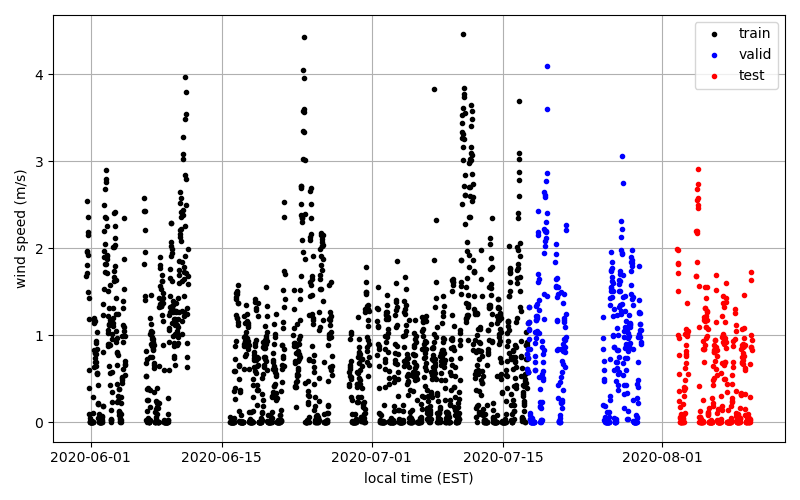
\includegraphics[width=0.49\textwidth]{temporal_sequence_wind_spd.png}
	}
	\hfill
	\subfloat[Solar Irradiance ($W/m^{2}$)\label{fig:sequence_temporal_e}]{
		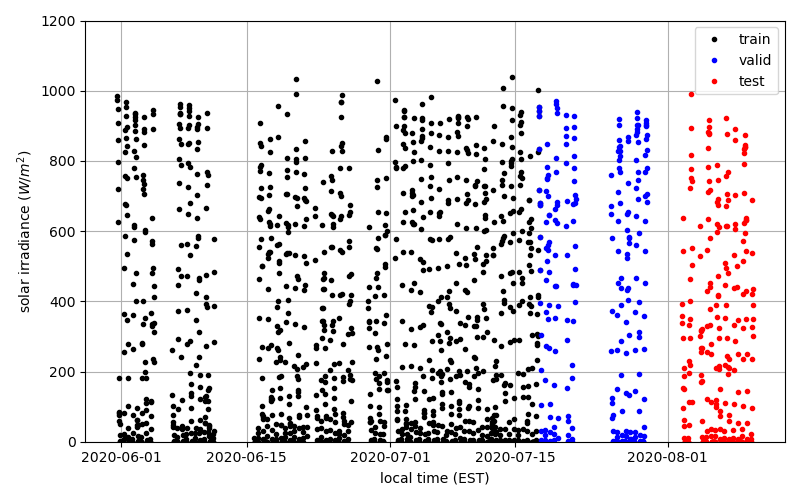
\includegraphics[width=0.49\textwidth]{temporal_sequence_solar_irr.png}
	}
	\subfloat[Turbulence $C_{n}^{2}$ ($m^{-2/3}$)\label{fig:sequence_temporal_f}]{
		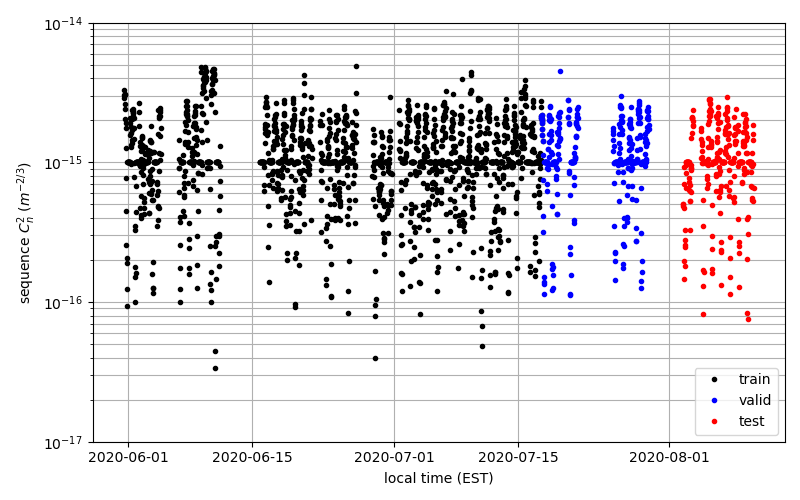
\includegraphics[width=0.49\textwidth]{temporal_sequence_cn2.png}
	}
	\hfill
	\caption{Sequence data as a function of time, parsed by train, validation, and test datasets drawn in black, blue, and red, respectively.}
	\label{fig:sequence_temporal}
\end{figure}

Histogram sequence plots presented in Figure \ref{fig:sequence_histograms}
\begin{figure}[p!]
	\centering
	\subfloat[Temperature (K)\label{fig:sequence_histograms_a}]{
		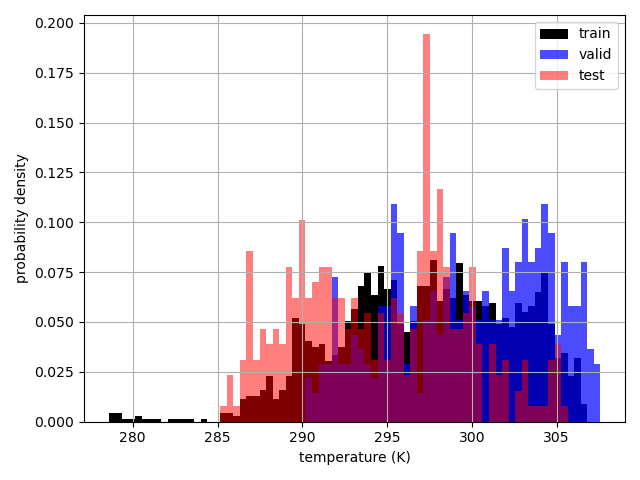
\includegraphics[width=0.49\textwidth]{hist_sequence_temp.png}
	}
	\subfloat[Pressure (Pa)\label{fig:sequence_histograms_b}]{
		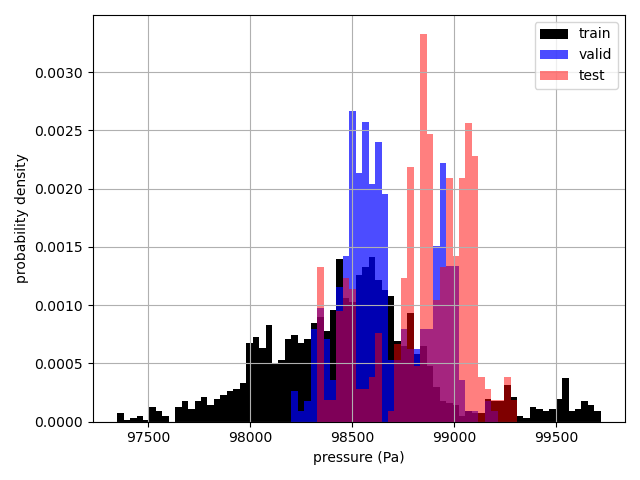
\includegraphics[width=0.49\textwidth]{hist_sequence_press.png}
	}
	\hfill
	\subfloat[Relative Humidity (\%)\label{fig:sequence_histograms_c}]{
	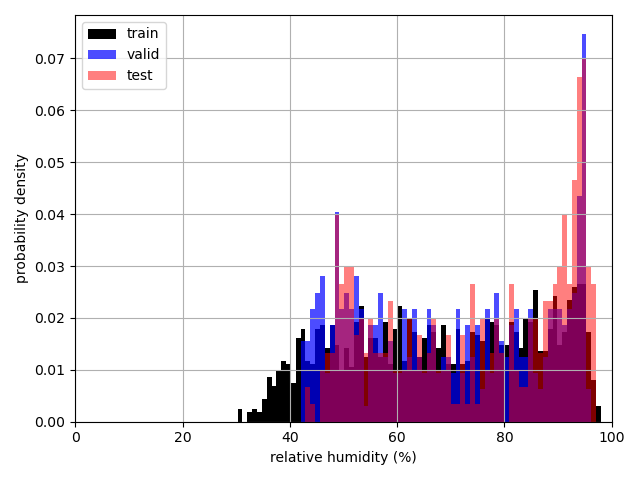
\includegraphics[width=0.49\textwidth]{hist_sequence_rh.png}
	}
	\subfloat[Wind Speed (m/s)\label{fig:sequence_histograms_d}]{
	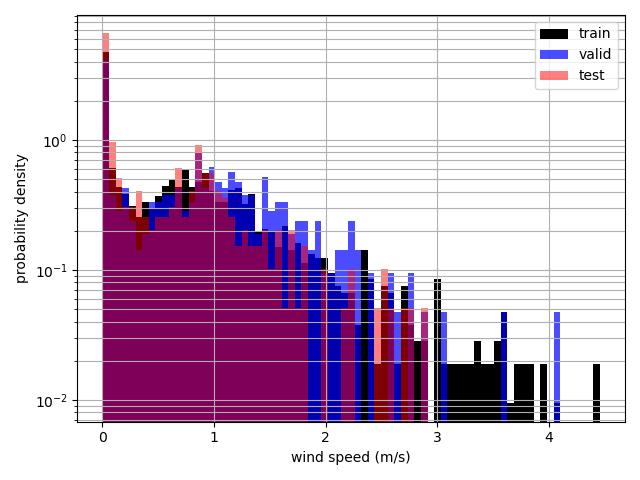
\includegraphics[width=0.49\textwidth]{hist_sequence_wind_spd.png}
	}
	\hfill
	\subfloat[Solar Irradiance\label{fig:sequence_histograms_e}]{
	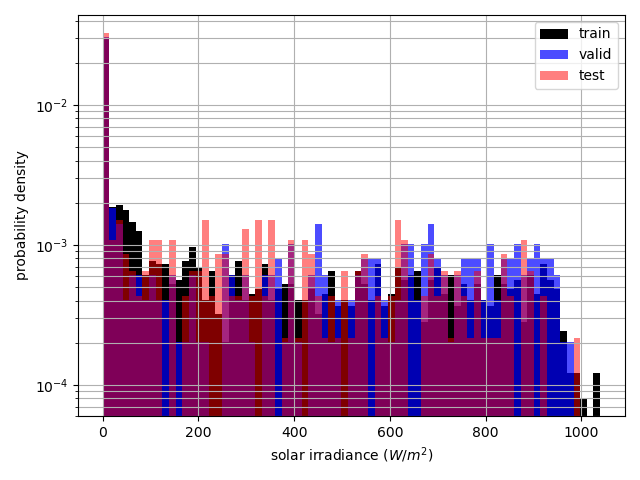
\includegraphics[width=0.49\textwidth]{hist_sequence_solar_irr.png}
	}
	\subfloat[$C_{n}^{2}$ ($m^{-2/3}$)\label{fig:sequence_histograms_f}]{
	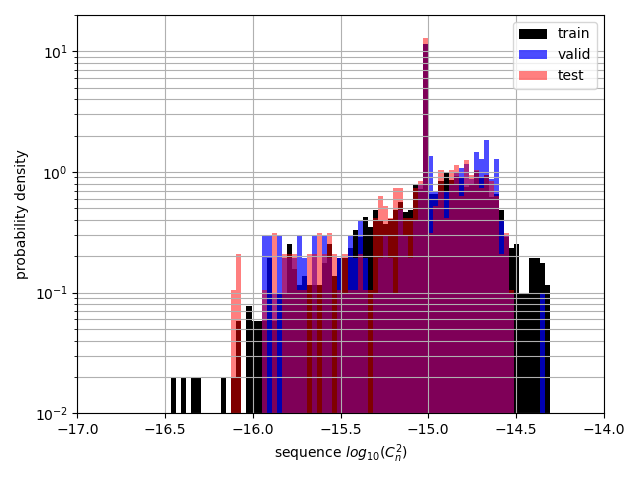
\includegraphics[width=0.49\textwidth]{hist_sequence_cn2.png}
	}
	\hfill
	\caption{Sequence data in normalized histograms, parsed by the train, validation, and test datasets drawn in black, blue, and red, respectively.}
	\label{fig:sequence_histograms}
\end{figure}

Forecast plots in Figure \ref{fig:forecast_sequence_histogram}
\begin{figure}[h!]
	\centering
	\subfloat[\label{fig:forecast_sequence_histogram_a}]{
		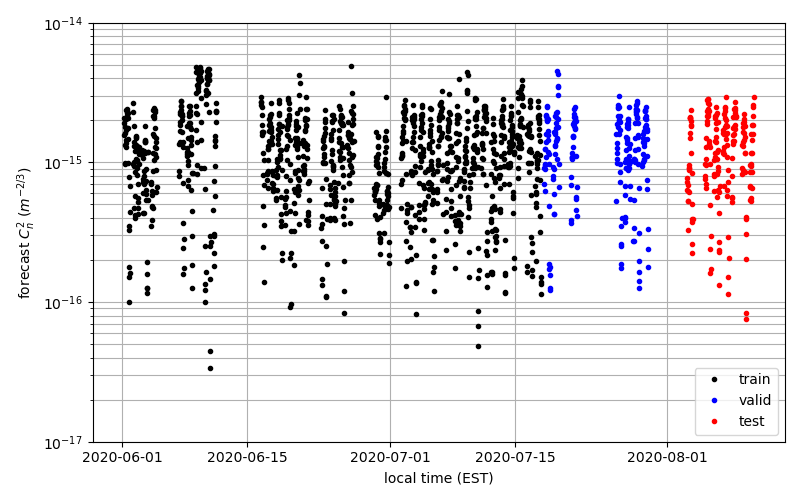
\includegraphics[width=0.543\textwidth]{temporal_forecast_cn2.png}
	}
	\subfloat[\label{fig:forecast_sequence_histogram_b}]{
		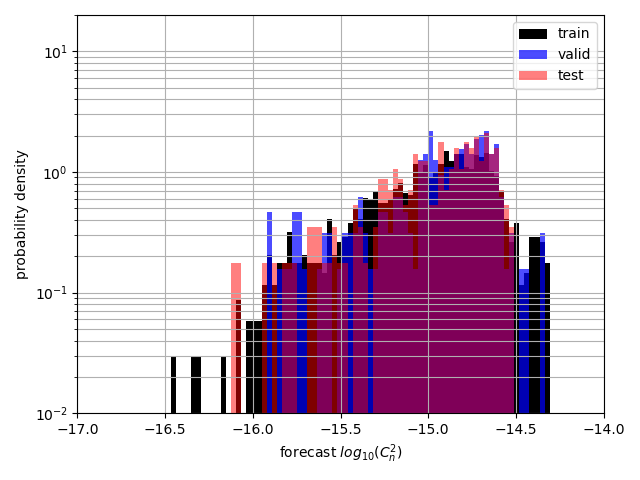
\includegraphics[width=0.447\textwidth]{hist_forecast_cn2.png}
	}
	\hfill
	\caption{Turbulence ($C_{n}^{2}$) forecasts as a function of time and as a normalized histogram. The train, validation, and test datasets are drawn in black, blue, and red, respectively.}
	\label{fig:forecast_sequence_histogram}
\end{figure}
\chapter{Grid Search}
\label{ch4}
This chapter walks through the methodology used to select the best model and parameters to forecast 4 hours of $C_{n}^{2}$ given prior environmental measurements, then the statistical analysis performed as a justification for the model selection.

\section{Methodology}
Given a problem to model with machine learning there are model hyperparameters to adjust in infinitely many combinations, each of which can impact model performance. Just a few examples of these hyperparameters are the optimization algorithm, the learning rate of the optimization algorithm, the number of layers in a model architecture and the number of nodes per layer. Given the many combinations of a model's hyperparameters, a careful method to determine the best combination must be employed. The definition of the ``best" model is the model which results in the best performance when applied to the validation dataset, a subset of the entire dataset specifically held from training for hyperparameter tuning. By holding back the validation dataset, an unbiased optimization of the hyperparemeters can be performed. The model and parameters which performs best on the validation dataset is then applied to the test dataset for another unbiased evaluation of the final model.

There are many methods of hyperparameter optimization, but common methods are grid search and random search. Grid search, or a parameter sweep, is an exhaustive search through manually specified hyperparameters. If iterating over only one hyperparameter, for example three different learning rates, three models are trained with the three learning rates. A model is trained with the first learning rate and it's performance on the validation dataset is recorded, then another model is trained but with the second learning rate and the performance on the validation dataset is recorded. This is done once more for the third learning rate. The performance of the models with the three learning rates are compared and the best learning rate is the learning rate used by the model that performed best. This method can quickly explode in computation time as the number of hyperparameters to iterate increases. For example, iterating over two hyperparameters of three values each results in nine combinations of hyperparameters. The number of combinations is defined as the multiple of the number of values across each hyperparameter, so if there are five hyperparameters with 1, 2, 3, 4, and 5 values, then the total number of combinations is $1 \times 2 \times 3 \times 4 \times 5 = 120$ combinations.

The other common method, the random search, replaces the exhaustive grid search by randomly selecting hyperparameters within defined bounds. An algorithm randomly selects the hyperparameters and models are trained with the different combinations then applied to the validation dataset to evaluate performance. A benefit of the random search is the selection of parameter combinations that might not be defined in a grid search.

In this work the grid search is employed because prior knowledge of hyperparameters is unknown, thus the exhaustive grid search is necessary to explore a wide range of combinations. This grid search iterates over five parameters. The outermost parameter is the four fundamental architectures: MLP, simple RNN, GRU, and LSTM. The MLP is a common machine learning architecture and serves as a baseline. The simple RNN, GRU, and LSTM are variants of the general RNN and are searched to find if a specific variant is better or worse than the others when applied to this problem. The next parameter is the input sequence variables used by the model. From Section \ref{sec:wx_seq_hist}, the available input sequence features (variables) are prior temperature, pressure, relative humidity, wind speed, solar irradiance, and $C_{n}^{2}$ measurements. The \textit{input features} parameter iterates over which features (variables) to train the model. Since there are six available features, and each feature can only be used or not used, there are $2^6 = 64$ total combinations. However, a threshold is set to train on a minimum of four features which reduces the total number of input feature combinations to 22. This threshold is set to discourage the model from memorizing one or two features, and for a significant reduction in computation time.

The third search parameter is the \textit{input sequence length}. Independent of the input features (variables), in a single sequence/forecast the amount of information available to the model is dependent on the time-length of the input sequence. Whether the model performs best with only 4 hours of input data or 16 hours of input data is highly relevant information. Thus, four lengths of the input sequence are searched: 4, 8, 12, and 16 hours. These lengths are chosen to be $1\times$, $2\times$, $3\times$, and $4\times$ the 4 hour forecast length. Note that the train, validation, and test datasets are carefully formatted so the same forecasts are trained, validated, and tested regardless of the input sequence length. This avoids an instance where a 4 hour input sequence might exist for a particular forecast but a 16 hour input sequence is not available due to missing data. The fourth parameter searched is the number of hidden layers in each architecture: 1 or 2. The fifth and final searched parameter is the number of hidden nodes per hidden layer: 10 through 50 in steps of 10. The final two parameters essentially search over the number of parameters in the model with some variation in the interaction of those parameters. Each fundamental architecture in total iterates over $22 \times 4 \times 2 \times 5 = 880$ combinations of parameters. Due to the stochastic nature of model training, a single model could perform significantly different than another model trained with the same parameters, thus a total of 10 models are trained per combination per fundamental architecture to ensure the stability of results. In this search a total of $880 \times 4 \times 10 = 35,200$ models are trained.

For each model trained in the grid search the following parameters are fixed: mini-batch size, optimization algorithm, initial learning rate, learning rate decay (step and decay factor), and weight decay. The mini-batch size, the number of training examples used per model parameter update, is set to 32 yielding a total of 30 parameter updates (933/32) per epoch (iteration through the entire dataset). The optimization algorithm is AdamW\cite{kingma2017adam} \cite{loshchilov2019decoupled}. The initial learning rate is 0.01 and decays by a factor of 10 every 10 epochs. This results in learning rates 0.01, 0.001, 1e-4, 1e-5, and 1e-6 from epochs 1 - 10, 11 - 20, 21 - 30, 31 - 40, and 41 - 50, respectively. The high initial learning rate is to ensure suitably-high gradients are back-propagated through the model to allow each model 10 epochs (300 total parameter updates) to escape any local minima. This training method consistently leads to a strong model convergence in only a few seconds. The weight decay is a regularization technique applied to the optimization algorithm and is 0.001.

\section{Grid Search Results}
The analyses of the grid search are performed independently on each architecture. From the four grid searches, four 2d-arrays of RMSE loss scores, the performance metric between validation truth and output $log_{10}(C_{n}^{2})$, are recorded for analysis. The 2d-arrays are shape $880 \times 10$ for 880 parameter combinations and 10 models each. From these four 2d arrays, the average and standard deviation of the RMSE scores are calculated per parameter combination yielding four arrays of 880 averages and standard deviations. The standard deviation, the square root of the average of the squared deviations from the mean, is calculated by
\begin{equation} \label{eq:standard_deviation}
	\sigma = \sqrt{\frac{\sum\left(x - \bar{x}\right)^{2}}{N - ddof}}
\end{equation}
where $\sigma$ is the standard deviation, $x$ is the data, $\bar{x}$ is the average of the data, N is the number of data points, and $ddof$ is the delta degrees of freedom. Using $ddof = 1$ provides an unbiased estimator of the variance of the infinite population. It is standard practice to use $ddof = 1$. $ddof = 0$ should be used in the situation of measuring the variance of a distaribution whose mean $\bar{x}$ is known a priori rather than being estimated from the data \cite{10.5555/1403886}.

If the average, $\bar{x}$ in Equation \ref{eq:standard_deviation}, were calculated many times with different sets of sampled data the values of $\bar{x}$ would themselves have a standard deviation. This is called the \textit{standard error} of the estimated mean $\bar{x}$. Assuming the underlying distribution is Gaussian, the \textit{standard error} is given approximately by
\begin{equation} \label{eq:standard_error}
	\sigma_{\bar{x}} = \frac{\sigma}{\sqrt{N}},
\end{equation}
where $\sigma_{\bar{x}}$ is the standard error of the mean, $\sigma$ is the standard deviation from Equation \ref{eq:standard_deviation}, and $N$ is the number of samples used the calculate $\bar{x}$ \cite{10.5555/1403886}. In the calculation of the standard error of the average loss scores, $N$ is 10, the number of models trained for each combination of the grid search. From these statistics the best model as applied to the validation dataset is determined and significance quantified.

\subsection{Results Sorting}
The four arrays of average RMSE scores are sorted from best to worst and the sort indices are applied to the array of grid search parameters. From these sorted arrays the best model and its parameters are extracted. Figure \ref{fig:grid_search_results} illustrates the validation average $log_{10}(C_{n}^{2})$ RMSE loss as a function of the sorted index. Figure \ref{fig:grid_search_results_a} plots all 880 sorted scores for each fundamental architecture. Figure \ref{fig:grid_search_results_b} plots only the first ten to focus on the best performers. In each plot MLP is drawn in blue, simple RNN in orange, GRU in green, and LSTM in red. The curves in each figure are monotonically increasing because the sorted losses are plotted. Figure \ref{fig:grid_search_results_b} additionally plots the standard error.
\begin{figure}[h!]
	\centering
	\subfloat[Full set of iterations\label{fig:grid_search_results_a}]{
		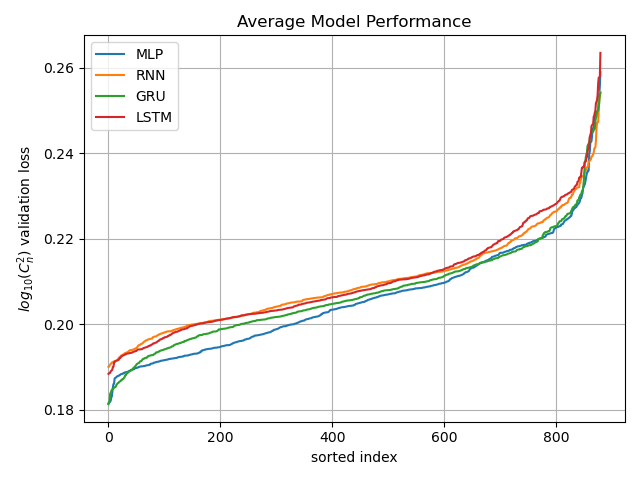
\includegraphics[width=0.49\textwidth]{average_model_performance_wide.png}
	}
	\subfloat[Top 10 iterations\label{fig:grid_search_results_b}]{
		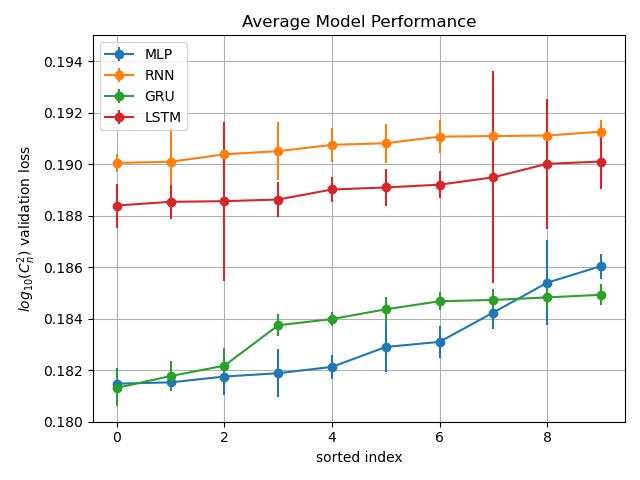
\includegraphics[width=0.49\textwidth]{average_model_performance_narrow.png}
	}
	\hfill
	\caption{Grid search results.}
	\label{fig:grid_search_results}
\end{figure}
The general shape of the sorted loss curves are highly correlated from architecture to architecture and their slopes are consistent from sorted index 100 through 800. On either side, between sorted indices 0 through 100, and 800 through 880, the curves exponentially increase. This is an indication that there are a general set of modeling parameters which are notably better than all the others, and likewise a set that are far worse than the others.

In terms of model performance, the curves in Figure \ref{fig:grid_search_results_a} generally indicate that over the grid search space the MLP dominates the ensemble of RNN architectures. Throughout the sorted indices, but most importantly at the beginning (left) of the sorted indices, the MLP (blue) and GRU (green) architectures perform better by a large margin compared with the simple RNN (orange) and LSTM (red) architectures. This is further shown in Figure \ref{fig:grid_search_results_b} which illustrates the first ten sorted indices of Figure \ref{fig:grid_search_results_a}. The loss curves illustrate that on average the best ten models of the simple RNN is the worst of the four architectures and the best ten models of the LSTM models are a small scale factor better. This result is interesting since the MLP is the baseline architecture and the ensemble of RNNs are designed to handle time series data. Another notable feature of the top ten LSTM models in Figure \ref{fig:grid_search_results_b} is the large standard error of the mean calculated from Equation \ref{eq:standard_error}. This is an indication of significant variance in performance over the 10 models trained per grid search iteration. During brief analysis two LSTM models trained on the same parameters could illustrate impressive then poor performance. This high variability is not desirable and leads to high average RMSE, but does reveal the capability of the LSTM if the right set of training parameters can consistently result in a good model.

Further evaluation of the loss curves in Figure \ref{fig:grid_search_results_b} shows that the best ten MLP and GRU models are very similar, even crossing each other twice. Of the top ten MLP and GRU models, the very best of each (sorted index 0) show that the GRU is slightly better with a validation average $log_{10}(C_{n}^{2})$ of 0.181316 vs. 0.181476 for the MLP. The standard errors are also very similar, 0.000697 vs. 0.000605, for the GRU and MLP, respectively. Thus the consistency of model convergence for one model is not notably better than the other. Generally the standard error bars of the MLP and GRU architectures in Figure \ref{fig:grid_search_results_b} are smaller (better) than the bars of the simple RNN and especially the LSTM architectures. These results illustrate that of the four architectures, the MLP and GRU are proving to be best suited for this problem as evaluated on the validation dataset.

\subsection{Statistical Significance}
The results presented in Figure \ref{fig:grid_search_results} clearly show that specific architectures and corresponding parameters perform better on the validation dataset than others. However, from the top performing models there is little discrepancy in performance metric which introduces ambiguity into which model and parameter combination is the very best. To sort through these similar models is the \textit{Student's t-test} which is a test of whether two sample means are different to a specific level of significance. Performing tests of significance on the results in Figure \ref{fig:grid_search_results_b} statistically distinguishes the models to show if a model is significantly better than another.

\subsubsection{\textit{Student's t-test} Foundation}
\label{sec:students_t-test}
The \textit{Student's t-test} is a statistical test of the null hypothesis $H_{0}$ that two samples have equal means. The alternative hypothesis $H_{a}$ is that samples do not have equal means. The foundation of the test is as follows. Take one set of measurements, then some event happens, then take another set of measurements. Did the event, like a change in a control parameter, make a difference? In this work the measurements are model performances on the validation dataset and the event is a change in the model parameters. There are several variations of the \textit{Student's t-test} including the \textit{independent t-test} for equal and unequal variances, and the \textit{dependent t-test} for paired samples. The \textit{independent t-test} for unequal variances is used in this work because the samples are independent and the variances are not assumed to be equal. This specific test is known as \textit{Welch's t-test} and given samples $x_{A}$ and $x_{B}$ defines the statistic \textit{t} as
\begin{equation} \label{eq:t_stat}
	t = \frac{\bar{x_{A}} - \bar{x_{B}}}{\sqrt{\frac{Var(x_{A})}{N_{A}} + \frac{Var(x_{B})}{N_{B}}}},
\end{equation}
where $\bar{x_{A}}$, $Var(x_{A})$ and $N_{A}$ are the sample A mean, variance and size, respectively. Likewise, $\bar{x_{B}}$, $Var(x_{B})$ and $N_{B}$ are the sample B mean, variance and size. The two-tailed $p$-value or significance of this value of \textit{t} is calculated with $dof$ degrees of freedom
\begin{equation} \label{eq:t_dof}
	dof = \frac{\left[\frac{Var(x_{A})}{N_{A}} + \frac{Var(x_{B})}{N_{B}}\right]^{2}}{\frac{\left[Var(x_{A})/N_{A}\right]^{2}}{N_{A} - 1} + \frac{\left[Var(x_{B})/N_{B}\right]^{2}}{N_{B} - 1}}.
\end{equation}
The $p$-value is a number between zero and one and is the probability that $|t|$ (hence two-tailed) could be this large or larger just by chance under the assumption that the null hypothesis $H_{0}$ is correct \cite{10.5555/1403886}. A very small p-value ($\le$ 0.05) means that the observed difference in means is very significant and the null hypothesis $H_{0}$ is rejected at the 5\% significance level. This does not, however, prove that the null hypothesis $H_{0}$ is false or the alternative hypothesis $H_{a}$ is true. A low $p$-value means \textit{either} that the null hypothesis is true and a highly improbable event has occurred \textit{or} that the null hypothesis is false.

\subsubsection{\textit{Student's t-test} Results}
The \textit{Student's t-test} described in above is robustly implemented as a function from \textit{SciPy}, a Python-based open-source software for mathematics, science, engineering, and most importantly in this case, statistics \cite{2020SciPy-NMeth}. Using the $ttest\_ind$ function and setting parameter $equal\_var$ to False performs the \textit{Welch's t-test} given two arrays of measurements.

The \textit{t-test} is performed on each of the top ten models in Figure \ref{fig:grid_search_results_b} where sample A in Equations \ref{eq:t_stat} and \ref{eq:t_dof} is the 10 validation $log_{10}(C_{n}^{2})$ RMSE scores from the very best GRU model. Sample B in Equations \ref{eq:t_stat} and \ref{eq:t_dof} iterates through the 10 validation RMSE scores of the rest of the models in Figure \ref{fig:grid_search_results_b}. This results in $p$-values of the best GRU model evaluated against the next nine best GRU models and the best ten MLP models, simple RNN models, and LSTM models. A significance level ($\alpha$) of 0.05 is predefined to reject the null hypotheses $H_{0}$ if the $p-$value is $\le \alpha$. Figure \ref{fig:students_t-test} summarizes these results by plotting the two-tailed $p$-value as a function of the sorted index, the same x-axis as in Figure \ref{fig:grid_search_results_b}. The $p$-values are again parsed by fundamental architecture.
\begin{figure}[h!]
	\centering
	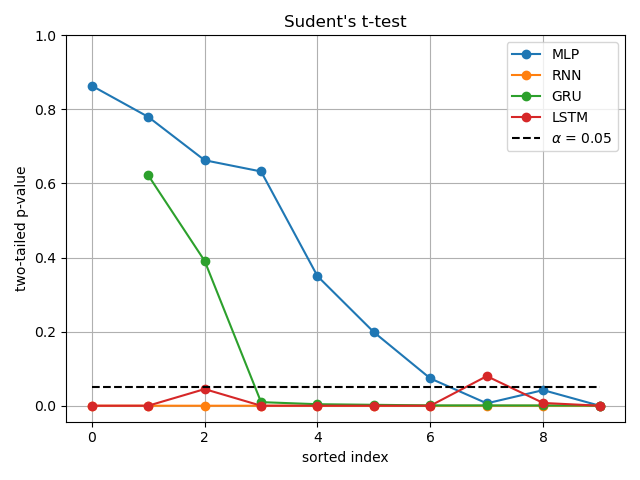
\includegraphics[width=0.7\textwidth]
	{students_t-test.png}
	\hfill
	\caption{\textit{Welch's t-test} of the grid search results}
	\label{fig:students_t-test}
\end{figure}
The MLP $p$-values are in blue, simple RNN in orange, GRU in green, and LSTM in red. The black dashed line in Figure \ref{fig:students_t-test} is the $p$-value threshold $\alpha = 0.05$. The GRU $p$-value at sorted index 0 (zero) is omitted because performing the \textit{Welch's t-test} on the best GRU model against itself is irrelevant.

Any markers below the black dashed line ($\alpha$) in Figure \ref{fig:students_t-test} represent models whose mean performance is statistically different from the best GRU model at the 5\% level, a rejection of the null hypothesis $H_{0}$. Since the best GRU model is the best performing model in the entire grid search, the models below the $\alpha$ line are statistically worse at the 5\% level. Any markers above the $\alpha$ line represent models whose performance is not statistically worse, i.e., the null hypothesis $H_{0}$ is not rejected at the 5\% level. A total of ten markers in Figure \ref{fig:students_t-test} are above the $\alpha$ line: two are the next two best GRU models, seven are the seven best MLP models, and one is the eighth best LSTM model. The LSTM model which does not reject the null hypothesis is a result of the high variance in the model illustrated by the large standard error bars in Figure \ref{fig:grid_search_results_b} at sorted index 8 on the x-axis. Likewise, the standard error bars at sorted index 3 in Figure \ref{fig:grid_search_results_b} also correspond with the $p$-value that is nearly to the $\alpha$ line in Figure \ref{fig:students_t-test}.

The other markers above the $\alpha$ line from MLP and GRU are consistent with the average RMSE scores in Figure \ref{fig:grid_search_results_b}. The first three GRU scores in Figure \ref{fig:grid_search_results_b} hover around 0.182 with the first three MLP scores. Then the GRU scores step up to nearly 0.184 and steadily increase. The MLP scores steadily rise until the seventh sorted index where there is a notable step above 0.184. The indices of these steps, three for GRU and seven for MLP, also are the first models where the null hypothesis is rejected at the 5\% level. This is illustrated in Figure \ref{fig:students_t-test} by the GRU (green) marker at sorted index 3 being the first GRU model below the $\alpha$ line and the MLP marker at sorted index 7 being the first MLP model below the $\alpha$ line.

\section{Evaluation of Best Models}
\subsection{Comparative Analysis}
From the results in Figure \ref{fig:students_t-test}, the top three GRU models and top seven MLP models are selected for further evaluation because they fail to reject the \textit{Welch's t-test} null hypothesis. The LSTM model which also does not reject the null hypothesis is not considered for further evaluation because its rejection is explained by the very high standard error. Mentioned above, the indices to sort the validation average $log_{10}(C_{n}^{2})$ RMSE scores are used to sort the corresponding grid search parameters. Table \ref{tab:grid_search_results_GRU} summarizes the grid search parameters associated with the top three GRU models.
\begin{table}[h!]
	\begin{center}
		\caption{Top GRU Model Parameters}
		\label{tab:grid_search_results_GRU}
		\begin{tabular}{||l|c|c|c|c||}
			\hline
			Model & Sequence Features & Sequence Length (hours) & Layers & Nodes \\
			\hline
			\hline
			GRU 1 & Press, RH, SI, $C_{n}^{2}$ & 12 & 2 & 40 \\
			\hline
			GRU 2 & Press, RH, SI, $C_{n}^{2}$ & 12 & 2 & 50 \\
			\hline
			GRU 3 & Press, RH, SI, $C_{n}^{2}$ & 12 & 2 & 30 \\
			\hline
		\end{tabular}
	\end{center}
\end{table}
The three rows in Table \ref{tab:grid_search_results_GRU} (ignoring the header) represent the best GRU model (GRU 1), then the next two best GRU models (GRU 2 and GRU 3). The columns in Table \ref{tab:grid_search_results_GRU} sort the grid search parameters into ``Sequence Features" which is the input sequence features (variables) used by the model, ``Sequence Length (hours)" that is the length of input sequence data used by the model and is reported in number of hours, ``Layers" which is the number of layers used by each model, and ``Nodes" which is the number of nodes per layer in each model.

The summary in Table \ref{tab:grid_search_results_GRU} is remarkably consistent. The input sequence features used by all three of the best models are pressure, relative humidity, solar irradiance and $C_{n}^{2}$, the sequence length of each model is 12 hours, the number of GRU layers for each model is two, and the number of nodes per GRU layer is 40, 50, and 30 in order of the top three GRU models. The consistency of the parameters from model-to-model indicates a specific type of model has been found to best perform on the validation dataset. It is also encouraging that the best GRU model uses 40 nodes per layer, then 50, and finally 30. If the best GRU used 50 nodes, for example, a concern would arise of whether the bounds of the grid search were wide enough, i.e., the number of nodes covered in the grid search have gone higher than 50.

Similarly to Table \ref{tab:grid_search_results_GRU}, Table \ref{tab:grid_search_results_MLP} summarizes the grid search parameters for the top seven MLP models.
\begin{table}[h!]
	\begin{center}
		\caption{Top MLP Model Parameters}
		\label{tab:grid_search_results_MLP}
		\begin{tabular}{||l|c|c|c|c||}
			\hline
			Model & Sequence Features & Sequence Length (hours) & Layers & Nodes \\
			\hline
			\hline
			MLP 1 & Temp, Press, RH, SI & 16 & 2 & 30 \\
			\hline
			MLP 2 & Temp, Press, RH, SI & 16 & 2 & 40 \\
			\hline
			MLP 3 & Temp, Press, RH, SI & 16 & 2 & 50 \\
			\hline
			MLP 4 & Temp, Press, RH, SI & 16 & 2 & 20 \\
			\hline
			MLP 5 & Temp, Press, RH, SI & 12 & 2 & 40 \\
			\hline
			MLP 6 & Temp, Press, RH, SI & 12 & 2 & 30 \\
			\hline
			MLP 7 & Temp, Press, RH, SI & 12 & 2 & 50 \\
			\hline
		\end{tabular}
	\end{center}
\end{table}
Evaluation of Table \ref{tab:grid_search_results_MLP} again yields consistency of the best MLP models. For each of the models the input sequence features are temperature, pressure, relative humidity, and solar irradiance. The input sequence length is 16 hours for the first four models, then 12 hours for the last three. The number of hidden MLP layers is two for all seven models. Finally, the number of nodes is 30, 40, 50, then 20 for the 16 hour sequence lengths (first four models), then 40, 30, and 50 for the 12 hour sequence lengths (last three models).

The consistency of input sequence features in the best MLP models is encouraging because like the best GRU models, a specific type of MLP model has been found to perform best on the validation dataset. It's also encouraging that the number of hidden layers in the MLP model is consistently 2 across all seven models. The ordering of the sequence lengths and number of nodes per hidden layer in Table \ref{tab:grid_search_results_MLP} illustrates that using 16 hours of input sequences and at least 20 nodes per layer is better than using 12 hours of input sequences and at least 30 nodes per layer. Most importantly, though, is shows that that using 12 hours of input sequences and at least 30 nodes is better than 16 hours of input sequences with only 10 nodes. This is an indication that using only 10 nodes per layer in the MLP likely does not yield the model complexity to perform well on the validation dataset.

There are two major distinctions between the best GRU and MLP models summarized in Tables \ref{tab:grid_search_results_GRU} and \ref{tab:grid_search_results_MLP}. First, the input sequences each only use four features (variables), but the features used by each architecture are different. Both architectures use pressure, relative humidity, and solar irradiance, but the GRU architecture uses $C_{n}^{2}$ and MLP uses temperature. It's interesting that the use of temperature, one of the most fundamental weather variables and oscillatory in character, is not used by the best GRU models. It's more interesting, however, that the best MLP models do not use prior $C_{n}^{2}$ measurements as an input. It's expected that the prior $C_{n}^{2}$ measurements would be a significant driver of the model outputs since generally the trend of recent measurements would continue in the future, so it's curious that the best MLP models deviate from this expectation. The second major distinction is the input sequence lengths. The best GRU models only require 12 hours of inputs, whereas the four best MLP models require 16 hours of inputs. From a practical perspective, requiring four less hours of input sequences is highly desirable in a real-world application.

In addition to the different input features used by the best GRU and MLP models, another curious result is that only four input features are used by each architecture when up to six variables are available. To investigate further, the ``Sequence Features" column in Tables \ref{tab:grid_search_results_GRU} and \ref{tab:grid_search_results_MLP} are expanded to evaluate more models, the best 88 (10\%) and worst 88 (10\%). The simple RNN and LSTM are also included in this analysis. The number of times each input feature (variable) is used by the best 88 and worst 88 models is recorded per architecture. Figure \ref{fig:variable_sets_analysis} illustrates bar charts of these results.
\begin{figure}[h!]
	\centering
	\subfloat[Best 10\%\label{fig:variable_sets_analysis_a}]{
		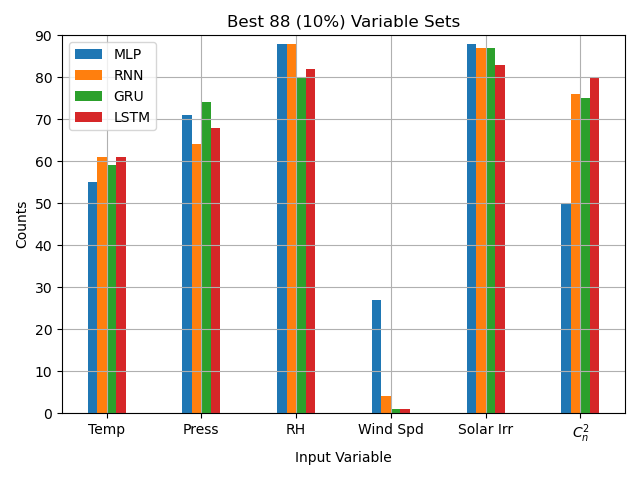
\includegraphics[width=0.49\textwidth]{bar_variable_sets_best.png}
	}
	\subfloat[Worst 10\%\label{fig:variable_sets_analysis_b}]{
		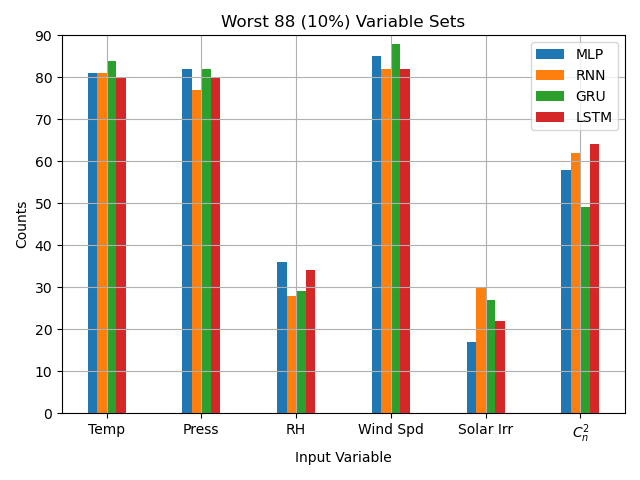
\includegraphics[width=0.49\textwidth]{bar_variable_sets_worst.png}
	}
	\hfill
	\caption{Best 10\% and worst 10\% variable sets.}
	\label{fig:variable_sets_analysis}
\end{figure}
Each category on the x-axis is an input feature, and the y-axis is the number of counts. There are four bars for each category representing the fundamental architectures. The blue bars are MLP, orange bars are simple RNN, green bars are GRU, and red bars are LSTM. Figure \ref{fig:variable_sets_analysis_a} is the counts of each input feature for the best 88 models of each architecture, and Figure \ref{fig:variable_sets_analysis_b} is the counts for the worst 88 models of each architecture.

Evaluation of best 88 models of each architecture in Figure \ref{fig:variable_sets_analysis_a} illustrates several interesting results, but one stands out in particular: wind speed is rarely used as an input feature in the best 10\% of models. Specifically, the ensemble of RNN architectures almost never use wind speed: the simple RNN uses wind speed four times, and the GRU and LSTM models only use wind speed once each. The best 88 MLP models, however, use wind speed just under 30 times. Concurrent evaluation of the worst 88 models of each architecture in Figure \ref{fig:variable_sets_analysis_b} further reveals information about wind speed: all four fundamental architectures use wind speed in nearly all of the worst 88 models. The ensemble of RNNs almost universally ignoring wind speed in the best models, combined with the almost universal inclusion in the worst models, is strong evidence that the exclusion of wind speed as an input feature for the best GRU and MLP models is not by chance. Rather, this is conclusive insight that prior wind speeds are not beneficial to the forecasting of $C_{n}^{2}$ in this problem. It is likely that this is due to the large spatial gap between the weather station and $C_{n}^{2}$ path. 

For the MLP, the wind speed counts in Figures \ref{fig:variable_sets_analysis_a} and \ref{fig:variable_sets_analysis_b} offer some insight into how the MLP is learning compared with the ensemble of RNN architectures. The processing of the RNNs essentially forces the model to learn the input sequences as a function of time, whereas the MLP, which uses the same information in a flattened layer, is free to learn any relationships. Specifically the MLP is not bounded to learn the temporal relationship between the input variables, thus is is reasonable to theorize that the MLP is more prone to learning relationships that are not as physical.

Two more categories of input features stand out in Figures \ref{fig:variable_sets_analysis_a} and \ref{fig:variable_sets_analysis_b}: relative humidity and solar irradiance are nearly universally used in the best 88 models of each architecture, and are seldom used in the worst 88 models of each architecture. This result reveals the opposite conclusion about wind speed: relative humidity and solar irradiance are strong drivers of $C_{n}^{2}$ and the spatial separation between weather measurements and $C_{n}^{2}$ path does not significantly impact the models' performances, i.e., these two variables are reliably transferred across space.

Temperature and pressure in Figures \ref{fig:variable_sets_analysis_a} and \ref{fig:variable_sets_analysis_b} are two input features whose counts require careful evaluation. In the best 88 models, temperature has an average around 57 - 58 counts across the four architectures, but has 80+ counts for each architecture in the worst 88 models. Similarly, pressure has around 68-69 counts on average in the best 88 models, and around 80 counts on average in the worst 88 models. The counts in the best 88 models suggest that pressure is not as sensitive to the problem as relative humidity and solar irradiance, and temperature is even less sensitive. The counts in the worst 88 models initially suggest that temperature and pressure are generally poor input features, but the very low counts of relative humidity and solar irradiance influence that conclusion, possibly incorrectly. Because a minimum of four input variables are required by the grid search's bounds, the low counts for relative humidity and solar irradiance already account for the maximum two dropped variables, which means that temperature and pressure by default will often get used as an input to the worst 88 models. This argument is not valid for wind speed because the counts are extremely low in the best 88 models \emph{and} the counts are extremely high in the worst 88 models. As a final note about temperature and pressure, if the minimum number of input features was set to three instead of four it's possible they would be entirely excluded from the best GRU models based on the counts in Figure \ref{fig:variable_sets_analysis_a}, leaving only relative humidity, solar irradiance, and $C_{n}^{2}$. 

The final input feature of discussion in Figures \ref{fig:variable_sets_analysis_a} and \ref{fig:variable_sets_analysis_b} is $C_{n}^{2}$. This is another input feature (wind speed) in which there is a strong difference between MLP and the ensemble of RNN architectures. For the best 88 models, $C_{n}^{2}$ is utilized 75+ times by the ensemble of RNN architectures, but only 50 times by the MLP. Most importantly, though, is that \emph{none} of the best seven MLP architectures from Table \ref{tab:grid_search_results_MLP} use $C_{n}^{2}$. This is further evidence of the fundamental difference between the processing of the ensemble of RNNs and the MLP. It's expected that prior $C_{n}^{2}$ measurements is a strong driver of future $C_{n}^{2}$ and the ensemble of RNNs strongly learn this relationship. The MLP has not learned this relationship as strongly possibly because $C_{n}^{2}$ is only relevant to forecasting $C_{n}^{2}$ if it is processed temporally.

The counts in Figures \ref{fig:variable_sets_analysis_a} and \ref{fig:variable_sets_analysis_b} have been shown to behave as a top-level input sensitivity analysis. Many useful conclusions have been derived about how the architectures use the inputs. Further evaluation would require a significant level of time-series analysis which is beyond the scope of this effort.

\subsection{Selection of the Best Model}
The results presented in this Chapter have shown the best performing model as applied to the validation dataset. By \textit{Welch's t-test} it has been shown to be significantly better than all but nine other models at the 5\% level. The best model (GRU) has been evaluated against the next two best GRU models to show strong consistency in the model parameters. This same evaluation and result has been shown for the seven MLP models. The next step in this work applies a model to the test dataset so a single model is chosen. This single model is ``GRU 1" in Table \ref{tab:grid_search_results_GRU}. It has two GRU layers with 40 nodes each and uses 12 hours of pressure, relative humidity, solar irradiance, and $C_{n}^{2}$ as input features. This model is chosen for many reasons.
\begin{enumerate}
	\item It results in the lowest average RMSE as applied to the validation dataset.
	\item The next two best GRU models, which are not significantly different in performance, share the same input features, input sequence length, and number of layers.
	\item This model uses 40 input nodes and the next two best GRU models, which are not significantly different in performance, use 50 and 30 nodes which shows strong consistency.
	\item This model requires only 12 hours of input sequences compared with MLP's requirement of 16 hours for the best models. In a real-world application this is highly desirable.
\end{enumerate}
In addition to the reasons to use the selected GRU model, no evidence has been shown to support the use of an MLP model instead.
\chapter{Test Results}
\label{ch5}

\section{GRU Test Dataset Performance Summary}
After determining the best model as applied to the validation dataset, the train and validation datasets are combined into an updated train dataset. The selected model is trained on the updated train dataset and then applied to the test dataset. Like in the grid search, 10 individual models are trained to evaluate convergence. Figure \ref{fig:GRU_train_test_loss_curves} illustrates the model training process by plotting the $log_{10}(C_{n}^{2})$ RMSE loss (evaluated between forecast and measured truth) as a function of training epoch. The blue curves represent each model's performance on the train dataset and the orange curves represent the performance on the test dataset. The solid and dashed black lines are the per-epoch average of the train and test dataset performances, respectively.
\begin{figure}[h!]
	\centering
	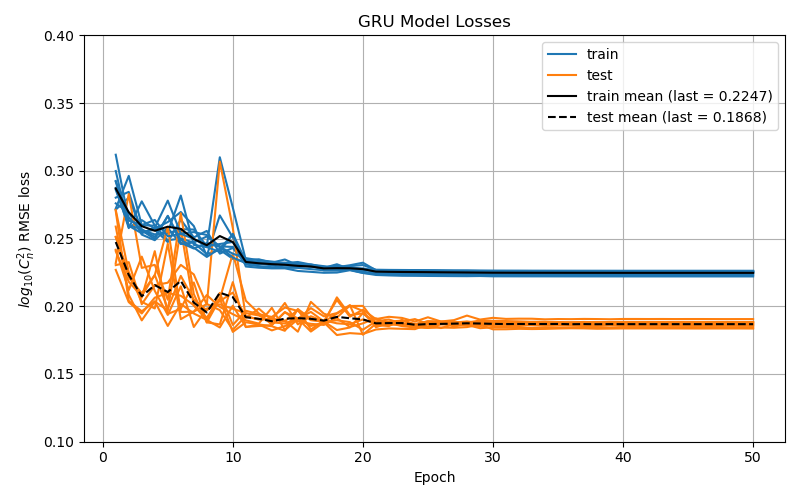
\includegraphics[width=0.75\textwidth]{GRU_loss_curves.png}
	\caption{GRU train and test loss curves of 10 models.}
	\label{fig:GRU_train_test_loss_curves}
\end{figure}
The loss curves in Figure \ref{fig:GRU_train_test_loss_curves} indicate that convergence rates of the models as applied to the train and test datasets are consistent with each other, an indication that the test dataset is a good representation of the train dataset. This is further illustrated by bumps in the loss scores in both train and validation loss curves like the single blue and orange spike at epoch 9. The per-epoch variability in the test dataset is higher than the train dataset since the test dataset is much smaller and thus more prone to changes in loss score with an update in model parameters. The 50th (last) epoch loss scores averaged over the 10 models are reported in the legend as 0.2247 and 0.1868 for the train and test dataset, respectively. The standard deviations of the 50th epoch loss scores for the train and test datasets are 0.0013 and 0.0020, respectively. As a point of comparison, the best MLP model was also trained then applied to the test dataset 10 times. The average 50th epoch loss scores are 0.2457 and 0.1938 with standard deviations of 0.0027990 and 0.0020191 for the train and test dataset, respectively. These results indicate that as applied to the test dataset, on average the chosen GRU model is better than the best MLP model by a large margin (\textcolor{blue}{add student's t-test p-value here to show significance?}), further validating the selection of the GRU model. The standard deviations of the test dataset loss scores are nearly identical, indicating the stability of the models are similar.

Another way to visualize model convergence is to apply the 10 individually-trained models to the test dataset parsed by day. The test dataset spans 08/03 and 08/05 - 08/10, so each model is evaluated on these seven days. The $log_{10}(C_{n}^{2})$ RMSE loss scores as a function of test day are illustrated in Figure \ref{fig:GRU_daily_performance}. Evaluated over the 10 models, in black is the mean, red the mean $\pm$ the standard deviation, and blue the minimum and maximum scores.
\begin{figure}[h!]
	\centering
	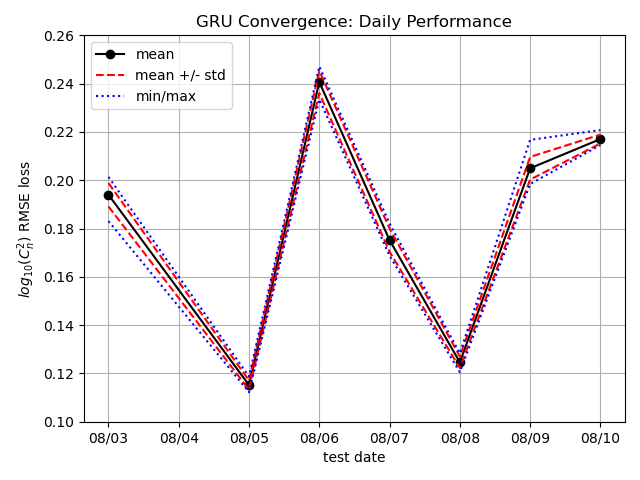
\includegraphics[width=0.65\textwidth]{GRU_daily_performance.png}
	\caption{GRU daily summary performance: mean, standard deviation, and min/max.}
	\label{fig:GRU_daily_performance}
\end{figure}
The day-to-day change in average error score, illustrated by the large jumps in error score like from 08/05 to 08/06, indicate that model performance varies by daily $C_{n}^{2}$ conditions. However, the tightness of the red and blue curves about the black markers indicate the models are converging to consistent solutions when evaluated on a daily basis. The largest difference between minimum and maximum loss scores is just less than 0.02 on 08/03 which is still a small variation in model performance for a given day. On 08/05 and 08/08 the red and blue lines are on top of the black markers indicating the model convergence is highly consistent when applied to these two days. These day-by-day results further confirm the test dataset loss curves in Figure \ref{fig:GRU_train_test_loss_curves} which indicate the models converge to a consistent solution when applied to the entire test dataset.

Another visualization of average model performance from the 10-model ensemble is presented in Figure \ref{fig:GRU_hourly_performance} which is the $log_{10}(C_{n}^{2})$ RMSE loss score of the test dataset parsed by the first timestep in each forecast. To make the plot in Figure \ref{fig:GRU_hourly_performance}, the 148 forecasts in the test dataset are sorted by the time of day of the first timestamp in each 4-hour forecast, the 30-minute forecast. The loss scores of each model applied to every test dataset forecast whose timestamp corresponds with a given time of day is plotted as the black markers. The average of the 10 loss scores are plotted as red markers for each test dataset forecast whose first timestamp is at the given time.
\begin{figure}[h!]
	\centering
	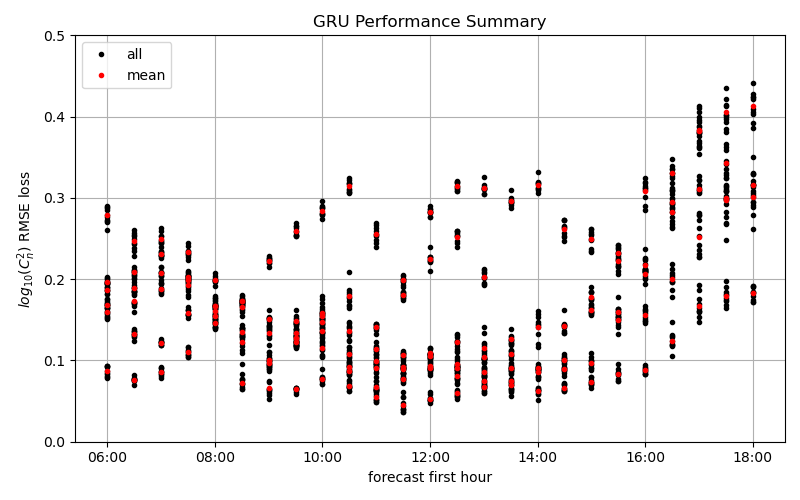
\includegraphics[width=0.65\textwidth]{GRU_hourly_performance.png}
	\caption{GRU hourly summary performance: individual and average.}
	\label{fig:GRU_hourly_performance}
\end{figure}
For example, evaluating the 06:00 (far left) time of day in Figure \ref{fig:GRU_hourly_performance} shows six red markers. This means that in the test dataset there are six forecasts whose first timestamp is at 06:00, and each red marker is the average loss (from the 10-model ensemble) for each of the six forecasts. The black dots at 06:00, of which there are 60 markers, are the model-by-model loss scores for each of the six forecasts. Still evaluating the 06:00 time of day, there is one red marker around 0.275 on the y-axis that is on top of a cluster of black points. This individual red marker is the average of the black markers which surround it. Thus, this cluster of black markers and their average, the red marker, is an evaluation of the ensemble model performance on one of the six forecasts whose first timestamp is at 06:00. Overall, Figure \ref{fig:GRU_hourly_performance} shows 148 red markers for the 148 forecasts in the test dataset, and 1480 black markers for the 10 models per 148 forecasts.

Figure \ref{fig:GRU_hourly_performance} is a summary of model performance as a function of time of day. The trends indicate that best model performance starts around 0.2 (on the y-axis) in the beginning of the day, drops down to around 0.1 in the middle of the day, then rises in the evening to around 0.3. The morning forecasts trend to be around the overall test dataset performance, about 0.18 to 0.20. On average, best performance is in the middle of the day between 11:00 and 15:00 since most of the black and red markers are clustered around 0.1 on the y-axis. In this window a few forecasts are consistently outliers (indicated by the red markers also being an outlier from the trend) in terms of error score. These individual forecasts are of interest for analysis. The high error scores at the end of the day, 16:00 to 18:00, is indicative that there are features of these late-day forecasts which are present in the measurements but are consistently not being captured by the ensemble of models. Generally, Figure \ref{fig:GRU_hourly_performance} indicates the model performs best in the middle of the day, slightly worse in the morning, and generally poorly in the late afternoon and evening.

\section{Daily $C_{n}^{2}$ Forecasts}
\label{sec:daily_cn2_forecasts}
After the ensemble study of the GRU models applied to the test dataset, a single GRU model is applied to the test dataset and carefully evaluated in this section. Figures \ref{fig:test_daily_results0} and \ref{fig:test_daily_results1} are daily-$C_{n}^{2}$ plots of the test forecasts and measured truth as a function of local time. Figures \ref{fig:test_daily_results0_a}, \ref{fig:test_daily_results0_b}, \ref{fig:test_daily_results0_c}, and \ref{fig:test_daily_results0_d} plot the forecasts on 08/03 and 08/05 - 08/07, respectively.  Figures \ref{fig:test_daily_results1_a}, \ref{fig:test_daily_results1_b}, and \ref{fig:test_daily_results1_c} plot the forecasts on 08/08 - 08/10, respectively. Each daily-$C_{n}^{2}$ plot contains multiple curves. The black curve represents the truth $C_{n}^{2}$ measured conditions. The other curves which transition in color from cyan to magenta represent the model forecasts throughout the day. The brightest cyan is the earliest forecast in the day, and the brightest magenta is the latest forecast in the day. The forecasts in between are appropriately colored to smoothly transition between the two end colors. The colorbar of each plot in Figures \ref{fig:test_daily_results0} and \ref{fig:test_daily_results1} illustrate the curve color scheme by labeling the forecast's first timestamp next to the color with which it's associated. Additionally, the $log_{10}(C_{n}^{2})$ RMSE loss score between each forecast and measured truth is also labeled in parenthesis next to the colorbars.
\begin{figure}[h!]
	\centering
	\subfloat[August 03\label{fig:test_daily_results0_a}]{
		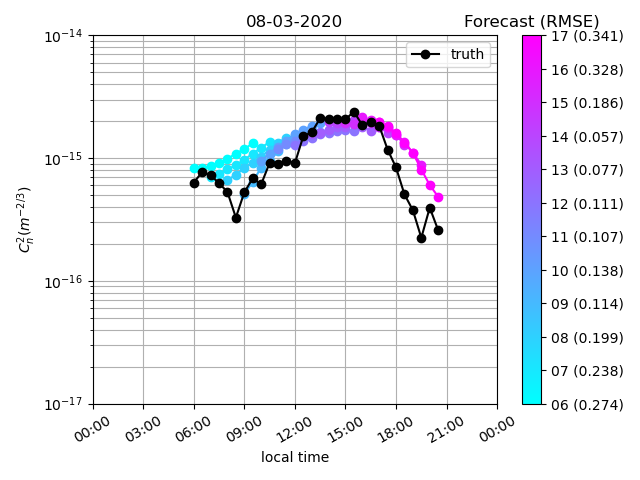
\includegraphics[width=0.49\textwidth]{forecasts_20200803.png}
	}
	\subfloat[August 05\label{fig:test_daily_results0_b}]{
		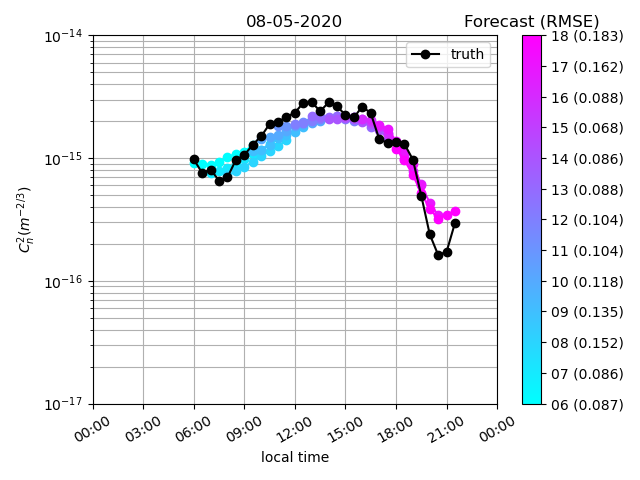
\includegraphics[width=0.49\textwidth]{forecasts_20200805.png}
	}
	\hfill
	\subfloat[August 06\label{fig:test_daily_results0_c}]{
		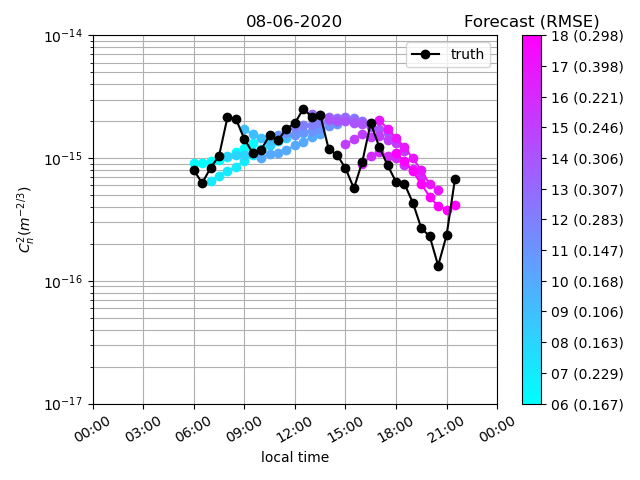
\includegraphics[width=0.49\textwidth]{forecasts_20200806.png}
	}
	\subfloat[August 07\label{fig:test_daily_results0_d}]{
		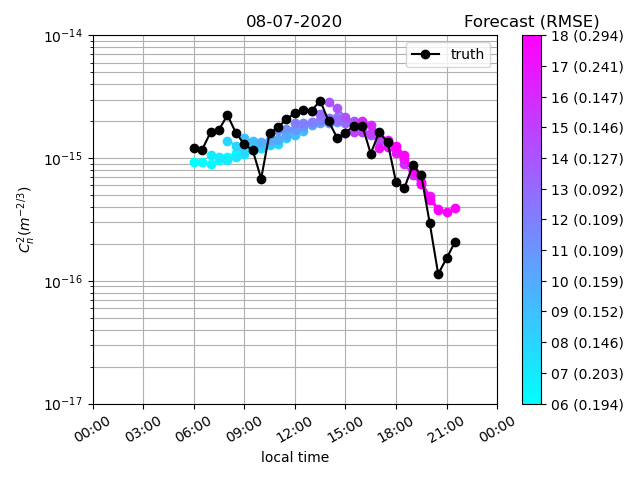
\includegraphics[width=0.49\textwidth]{forecasts_20200807.png}
	}
	\hfill
	\caption{August 3 and 5 - 7 daily $C_{n}^{2}$ forecasts.}
	\label{fig:test_daily_results0}
\end{figure}
For example in Figure \ref{fig:test_daily_results0_a}, the earliest forecast's (furthest left) first timestamp is at 06:00 and is correspondingly labeled in the colorbar as 06. The color of this earliest curve is brightest cyan which is consistent with the label on the colorbar. The error score for this forecast is 0.274. Likewise, the last forecast of the day in Figure \ref{fig:test_daily_results0_a} is at 17:00 and is the brightest magenta curve. The colorbar label is 17 and is the top color in the colorbar. The loss score for this individual forecast is 0.341. Note that in these daily-$C_{n}^{2}$ plots only the forecasts whose first timestamp is at the top of the hour are illustrated. This is done purely for aesthetics to avoid cluttered plots.

The daily-$C_{n}^{2}$ plots in Figure \ref{fig:test_daily_results0} illustrate many unique features. Starting with 08/03 in Figure \ref{fig:test_daily_results0_a}, the morning (cyan) forecasts all forecast a similar trend in $C_{n}^{2}$: a steady rise. Interestingly, the magnitude of the forecasted conditions seems to be different by a scale-factor between the first three forecasts at 06:00 - 08:00. This illustrates the impact of including prior $C_{n}^{2}$ conditions as an input sequence into the model. At the 07:00 and 08:00 forecasts, the model is given information that the most recently measured $C_{n}^{2}$ is trending down in magnitude so the forecasts, while still trending upward, lowers in overall magnitude because the model has learned that its forecasts should start near the most recently measured conditions. This feature is consistently seen throughout all test forecasts. Another interesting feature is the evening forecasts in Figure \ref{fig:test_daily_results0_a}. The 15:00 - 18:00 model forecasts predict $C_{n}^{2}$ to significantly lower in magnitude starting around 18:00 until 20:30. The measured conditions significantly lower, but temporally earlier than predicted. This is a rare case where the model gets the evening neutral event magnitude mostly right but misses the temporal component. Generally, the model on this day forecasts a mostly standard diurnal trend, but the measurements are weather impacted. At 10:00 there is a slight drop in measured turbulence, then from 10:30 - 12:00 the measured conditions are steady around $9 \times 10^{-16} (m^{-2/3})$. A standard diurnal trend occurs from 12:30 to 17:00, and the model accurately forecasts this.

Forecasts on 08/05 in Figure \ref{fig:test_daily_results0_b} are consistent with a standard diurnal trend. Specifically, the forecasts accurately predict the weak morning neutral event indicated by the drop in $C_{n}^{2}$ around 07:00 to 08:00 then a steady rise in strength until 12:00. The forecasts predict slightly lower $C_{n}^{2}$ strength than measured, but the difference is small. The forecasts then accurately predict the drop in $C_{n}^{2}$ strength starting around 15:00. These forecasts are accurate temporally and in strength of neutral event until the deepest part around 21:00. The measured $C_{n}^{2}$ strength continues to drop but the model does not reach this depth. However, the model does accurately forecast the slight rise in $C_{n}^{2}$ at the very end of the day. Every forecast in Figure \ref{fig:test_daily_results0_b} has an error score lower than the error score of 0.1868 from the 10-model ensemble average as applied to the entire test dataset. More specifically, 6 of the 12 forecasts have error scores less than 0.01. These scores indicate that 08/05 is an illustration of great model performance for an entire day.

Model performance on 08/06 in Figure \ref{fig:test_daily_results0_c} is the worst of the seven test days (see Figure \ref{fig:GRU_daily_performance}). The first three forecasts of the day at 06:00 - 08:00 have average to above-average error scores because the forecasts predict a steady rise in $C_{n}^{2}$ strength which generally is measured, but a weather-induced rise in $C_{n}^{2}$ strength at 08:00 is not captured. The 09:00 forecast, which boasts the lowest error score of the day of 0.104, benefits from knowledge of the prior $C_{n}^{2}$ measurements as an input. The forecast starts high, around $2 \times 10^{-15} (m^{-2/3})$, drops down in $C_{n}^{2}$ strength then continues upward in $C_{n}^{2}$ strength with the other forecasts which is accurate with the truth measurements. Forecast performance is poor again starting at 14:00 because another weather-induced turbulence event has occurred, but this time it's a 2-hour drop in $C_{n}^{2}$ strength which the forecasts beforehand do not predict. The 15:00 forecast is the first to see the prior measured $C_{n}^{2}$ conditions which include the weather event and so the model tries to compensate for the suddenly-lower $C_{n}^{2}$ strength by starting lower then rising for a few timestamps to reach the conditions it expects around this time. The 16:00 forecast captures the first timestamp, but misses the very high strength $C_{n}^{2}$ at 15:30, then sharp and consistent drop in $C_{n}^{2}$ as part of the evening neutral event from 15:30 till 20:30. The 17:00 and 18:00 forecasts also miss this long and deep evening neutral event. Overall, 08/06 illustrates where the model struggles: highly-weather impacted conditions.

The fourth test day, 08/07 in Figure \ref{fig:test_daily_results0_d}, illustrates a unique combination of forecasts. In the morning, the model forecasts a slow rise in $C_{n}^{2}$ strength until around 13:00 which is generally consistent with measurements, but does not predict the weather-induced rise in $C_{n}^{2}$ at 08:00 then subsequent drop at 10:00. These two events are very short, only consisting of a single timestamp (30 minutes). After this mini-event, the measured conditions are generally diurnal trend through 19:00. There are a few dips in measured $C_{n}^{2}$ strength but they are high frequency and bounce back to a normal diurnal trend which the model accurately forecasts. The forecasts from 11:00 through 16:00 all have error scores below 0.15, well below the average on the entire test dataset of 0.1868 from the ensemble results. The forecasts at 17:00 and 18:00 have high error scores because the model does not accurately predict the extremely sharp drop in $C_{n}^{2}$ strength from $7 \times 10^{-16} (m^{-2/3})$ at 19:30 to about $1 \times 10^{-16} (m^{-2/3})$ at 20:30, only 1 hour later. These late forecasts accurately predict the slight rise in turbulence at 21:00 and 21:30 after the deepest part of the evening neutral event, but the error scores are high because the model could not reach the depth. The 18:00 forecast is a good example of the model accurately forecasting the temporal nature of turbulence conditions but missing the very low magnitude of the neutral event.

The final three test days, 08/08 - 08/10, are presented in Figures \ref{fig:test_daily_results1_a}, \ref{fig:test_daily_results1_b}, and \ref{fig:test_daily_results1_c}, respectively. On average over the 10-model ensemble study, 08/08 is the second best day of model performance. Throughout the day, the model generally predicts diurnal trend: a slow rise in $C_{n}^{2}$ strength until around 15:00 where conditions steady then start to decrease again. The 09:00 through 13:00 forecasts all yield low error scores with 4 of them below 0.01. The first three forecasts from 06:00 through 08:00 have error scores around the ensemble average due to two factors. The 06:00 forecast first predicts turbulence conditions around $1 \times 10^{-15} (m^{-2/3})$, which is the nighttime filled $C_{n}^{2}$ strength, when the measured conditions are actually low. Then the 06:00 forecast altogether misses the weather-induced sharp rise in turbulence conditions from 07:00 to 08:30. The 07:00 and 08:00 forecasts also miss this high-frequency event. It's not until the 09:00 forecast which has the information about the prior turbulence conditions that the forecasts accurately settle into the diurnal trend.
\begin{figure}[h!]
	\centering
	\subfloat[August 08\label{fig:test_daily_results1_a}]{
		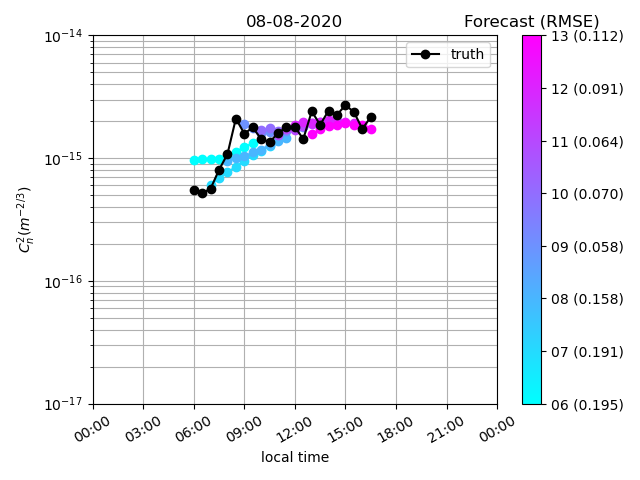
\includegraphics[width=0.49\textwidth]{forecasts_20200808.png}
	}
	\subfloat[August 09\label{fig:test_daily_results1_b}]{
		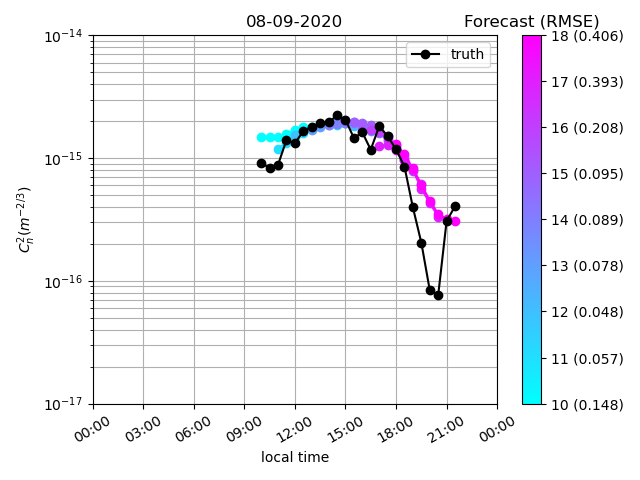
\includegraphics[width=0.49\textwidth]{forecasts_20200809.png}
	}
	\hfill
	\subfloat[August 10\label{fig:test_daily_results1_c}]{
		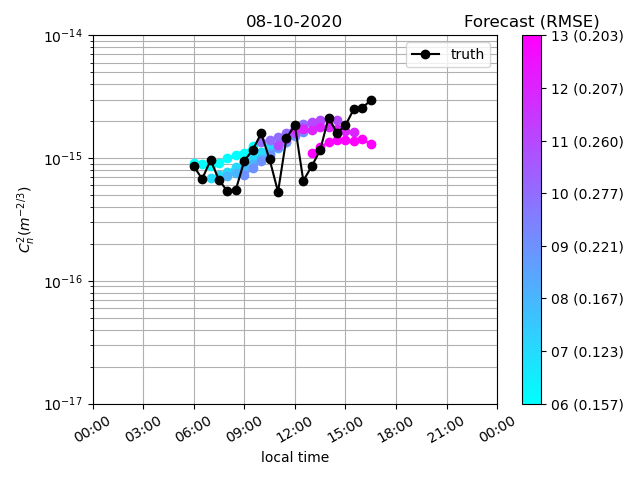
\includegraphics[width=0.49\textwidth]{forecasts_20200810.png}
	}
	\hfill
	\caption{August 8 - 10 daily $C_{n}^{2}$ forecasts.}
	\label{fig:test_daily_results1}
\end{figure}

From the 10-model ensemble study, model performance on 08/09 ranks 4/7 on average and is also one of the most variable from model-to-model (Figure \ref{fig:GRU_daily_performance}). Analysis of the forecast $C_{n}^{2}$ conditions in Figure \ref{fig:test_daily_results1_b} illustrate how an average over the entire day can be misleading. The first forecast at 10:00 has an error score of 0.148 which is below the 10-model overall average, then the 11:00 - 15:00 forecasts each boast error scores less than 0.01.The measured conditions are mostly diurnal and is accurately forecasted by the model. The only deviations are the very slight morning neutral event from 10:00 to 11:00 then a weather-induced slight drop in $C_{n}^{2}$ strength around 16:00. The two forecasts which raise the day's average error score are at 17:00 and 18:00. These forecasts accurately predict the temporal nature of the evening neutral event, but strongly miss the sharp decline and depth of the event. From 18:00 to 20:00, $C_{n}^{2}$ strength drops from just over $1 \times 10^{-15} (m^{-2/3})$ to $8 \times 10^{-17} (m^{-2/3})$, over 1 order-of-magnitude change. In fact, this evening neutral event is just one of only a handful of cases in the entire dataset in which the evening neutral event dips below $1 \times 10^{-16} (m^{-2/3})$ (\textcolor{blue}{count number of individual evening neutral events that reach this threshold? I think there are 7 including test dataset from Figure \ref{fig:forecast_sequence_histogram_a}}). The 17:00 and 18:00 forecasts yield error scores of 0.393 and 0.406, respectively, which are the two highest error scores in the entire test dataset. Beside this uncharacteristically deep neutral event, model performance on 08/09 is well better than average.

The last day of the test dataset, 08/10, is the second worst day of model performance from the 10-model ensemble average in Figure \ref{fig:GRU_daily_performance}. The morning forecasts, which begin at 06:00, generally all predict standard diurnal trends: a slow increase in $C_{n}^{2}$ strength through about 15:00 then a decline. The measured conditions, however, are highly variable both temporally and in $C_{n}^{2}$ strength. Between 06:00 and 15:00 there are five instances of a drop in $C_{n}^{2}$ strength. Likely, at least four of them are weather-induced (possible the 08:00 is morning neutral event). The model forecasts a diurnal trend which follows the trend of the high-strength $C_{n}^{2}$ points over this time period. The 12:00 and 13:00 forecasts predict $C_{n}^{2}$ strength to lower as the afternoon moves into early evening, but the measured conditions actually rise to the highest point in the entire day from 15:30 to 16:30. The 13:00 forecast starts at a lower $C_{n}^{2}$ strength than the surrounding forecasts due to the model having the input sequence information about the very low $C_{n}^{2}$ strength at 12:30. This day again illustrates the the model's inability to accurately forecast high-frequency weather-induced $C_{n}^{2}$ fluctuations. Instead, the model has learned a trend in $C_{n}^{2}$ based on the time of day. The model has also learned to adjust its starting $C_{n}^{2}$ strength based on prior $C_{n}^{2}$ measurements, then settle back into the expected trend. 

\section{Forecast Analysis}
The model forecasts and corresponding truth measurements from Figures \ref{fig:test_daily_results0} and \ref{fig:test_daily_results1} are rearranged by forecast length. Figure \ref{fig:test_scatter_results} presents a scatter plot of measured $C_{n}^{2}$ on the x-axis and forecasted $C_{n}^{2}$ on the y-axis for each time in the 4-hour model forecasts: 0.5 hour, 1 hour, 1.5 hour, and so on through 4 hours. In each scatter plot, the black markers are the truth values plotted as measured $C_{n}^{2}$ vs. measured $C_{n}^{2}$ to yield the linearly arranged markers. The green markers are the model forecast at the scatter plot's designated forecast time plotted as forecasted $C_{n}^{2}$ vs. measured $C_{n}^{2}$.
\begin{figure}[p!]
	\centering
	\subfloat[\label{fig:test_scatter_results_a}]{
		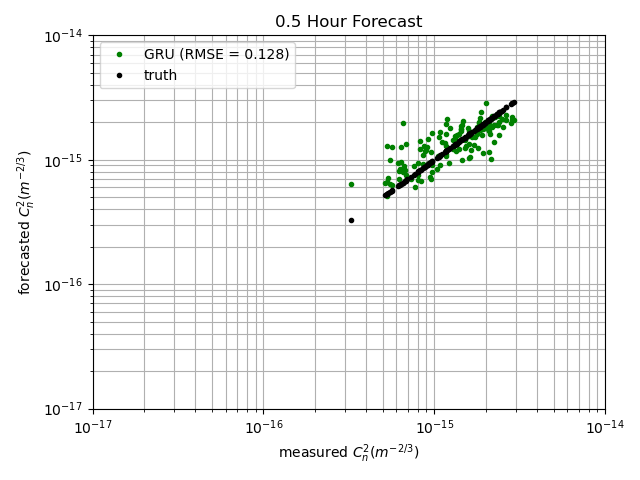
\includegraphics[width=0.40\textwidth]{scatter_0p5hr.png}
	}
	\subfloat[\label{fig:test_scatter_results_b}]{
		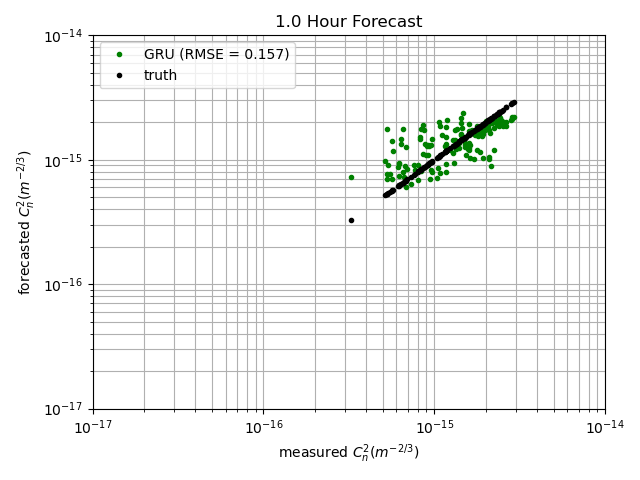
\includegraphics[width=0.40\textwidth]{scatter_1p0hr.png}
	}
	\hfill
	\subfloat[\label{fig:test_scatter_results_c}]{
		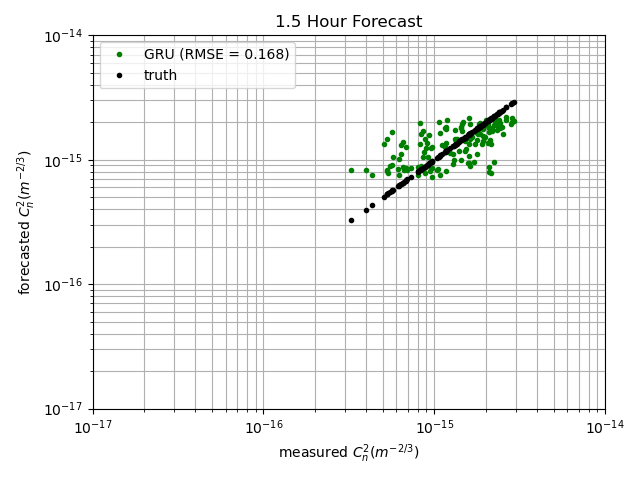
\includegraphics[width=0.40\textwidth]{scatter_1p5hr.png}
	}
	\subfloat[\label{fig:test_scatter_results_d}]{
		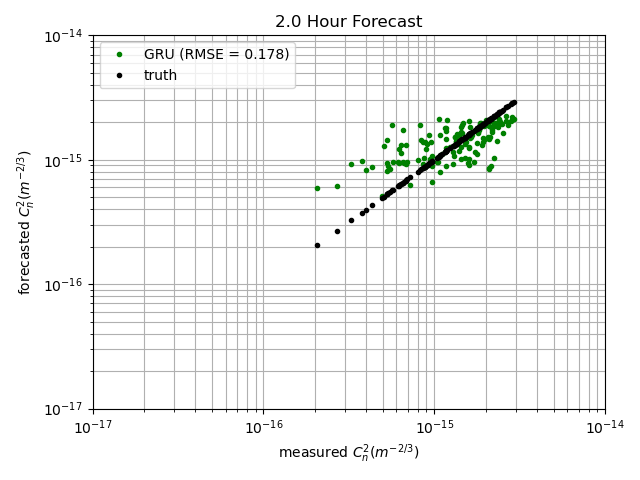
\includegraphics[width=0.40\textwidth]{scatter_2p0hr.png}
	}
	\hfill
	\subfloat[\label{fig:test_scatter_results_e}]{
		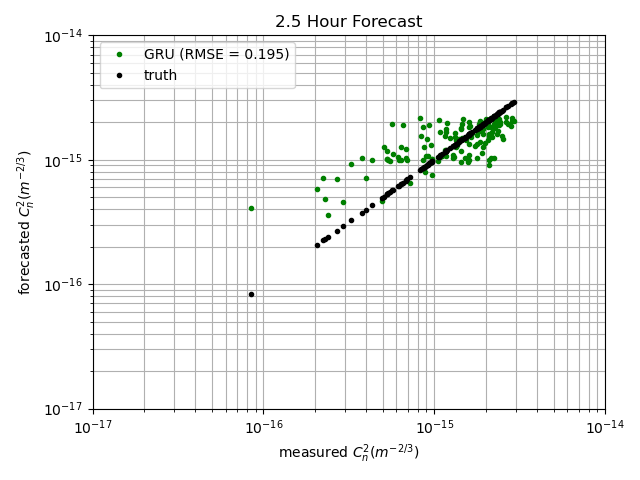
\includegraphics[width=0.40\textwidth]{scatter_2p5hr.png}
	}
	\subfloat[\label{fig:test_scatter_results_f}]{
		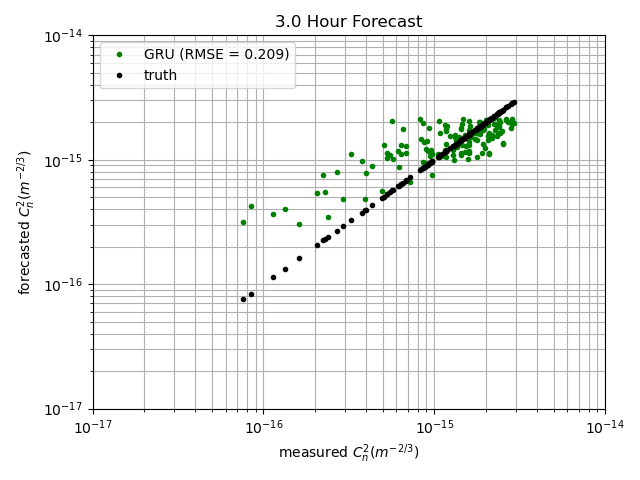
\includegraphics[width=0.40\textwidth]{scatter_3p0hr.png}
	}
	\hfill
	\subfloat[\label{fig:test_scatter_results_g}]{
		\includegraphics[width=0.40\textwidth]{scatter_3p5hr.png}
	}
	\subfloat[\label{fig:test_scatter_results_h}]{
		\includegraphics[width=0.40\textwidth]{scatter_4p0hr.png}
	}
	\hfill
	\caption{Scatter plots.}
	\label{fig:test_scatter_results}
\end{figure}
These scatter plots are visually evaluated by how closely the green markers cluster around the black markers. A set that is well clustered around the black points is better than a set that is not well clustered. If the model was perfect, the black markers would directly overlay the green markers. As a quantitative metric of model performance at each forecast hour the average $log_{10}(C_{n}^{2})$ RMSE loss is reported in each legend.

The scatter plot of the first forecast time, 30 minutes, in Figure \ref{fig:test_scatter_results_a} shows a strong clustering of the model forecasts about the measured $C_{n}^{2}$. Excluding one outlier, the range of measured $C_{n}^{2}$ the model is tasked to forecast is only from $5 \times 10^{-16} (m^{-2/3})$ to $3 \times 10^{-15} (m^{-2/3})$, a narrow window. This forecast time also benefits from being closest to the most recently measured $C_{n}^{2}$ and other input sequence variables. Thus, it is expected for this forecast time to do well overall. The RMSE loss score is 0.128, well below the 10-model ensemble average over the whole dataset of 0.1868. The scatter plot of the second time of the model forecasts, 1 hour, in Figure \ref{fig:test_scatter_results_b} shows a slightly worse performance than the 30 minute forecast time. The set of measured points looks very similar to that of 30 minutes, but the clustering of the green model markers about the black truth markers is not as tight. The error score of 0.157 confirms this visual analysis.

The 1.5 and 2 hour forecasts in Figures \ref{fig:test_scatter_results_c} and \ref{fig:test_scatter_results_d} start to clearly show a different set of measured $C_{n}^{2}$ conditions illustrated by the additional black markers toward the middle and lower left corner of the scatter plots. Most of the green model markers have a reasonable cluster around the mid- and high-strength $C_{n}^{2}$ black markers. However, the model struggles to capture measurements below $7 \times 10^{-16} (m^{-2/3})$ as illustrated by the black markers continuing left on the x-axis below this strength, but the green markers staying above $7 \times 10^{-16} (m^{-2/3})$ on the y-axis in Figure \ref{fig:test_scatter_results_c}. In Figure \ref{fig:test_scatter_results_d} is a similar trend, but a couple of model points are beginning to drop into lower strength $C_{n}^{2}$ conditions. The average error scores continue to climb, reaching 0.168 and 0.179 at the 1.5 and 2 hour forecast times, respectively.

The 2.5 and 3 hour forecasts in Figures \ref{fig:test_scatter_results_e} and \ref{fig:test_scatter_results_f} further shown a different set of measurements the model attempts to forecast. Most notable are the increased number of low-strength $C_{n}^{2}$. As forecast time extends further out the number of evening neutral events included in the examined sets also increases. The clustering of the higher-strength $C_{n}^{2}$ conditions continues to slightly deteriorate. The clustering of the green model markers is not as tight about the black truth markers, and more importantly the slope of these green markers is angling more with respect to the slope of the black markers. At low-strength $C_{n}^{2}$ evening neutral events the model is still struggling to forecast $C_{n}^{2}$ that reaches the measured strength. One positive element of these scatter plots is that there are no green markers which are wildly off from it's corresponding black marker. For example, there are no green modeled markers at $2 \times 10^{-15} (m^{-2/3})$ when it's black marker is nearing $1 \times 10^{-16} (m^{-2/3})$. This means the model has generally learned the turbulence conditions well, understanding when to forecast high, medium, and low-strength $C_{n}^{2}$. The error scores for the 2.5 hour and 3 hour forecasts are 0.197 and 0.211, respectively, which follows the trend of increasing error with forecast length.

Finally, the 3.5 and 4 hour forecasts in Figures \ref{fig:test_scatter_results_g} and \ref{fig:test_scatter_results_h} continue to illustrate the trend shown so far: the set of measured $C_{n}^{2}$ to forecast further evolves to include more evening neutral event low-strength conditions. Interestingly, the group of green model markers around the higher-strength $C_{n}^{2}$ is very well clustered with itself, but is at a significant angle with respect to the black truth markers' angle. The model's struggle to capture the deep neutral events is most clearly observed in Figures \ref{fig:test_scatter_results_g} and \ref{fig:test_scatter_results_h}. The model still has learned when to forecast low-strength $C_{n}^{2}$, but cannot reach the required depth. The average loss scores for the 3.5 and 4 hour forecasts are 0.212 and 0.214, respectively.

%The lowest-strength $C_{n}^{2}$ forecasted by the model in the entire test dataset is $3 \times 10^{-16} (m^{-2/3})$ when there are multiple measurements weaker than this level.

Summarizing the scatter plot error scores from Figure \ref{fig:test_scatter_results} is Figure \ref{fig:performance_forecast_length} which plots the loss scores as a function of forecast length. The plot illustrates that as the forecast length increases so does the model performance error. This is an expected result as any forecasting application is expected to decline in performance as forecast time increases.
\begin{figure}[h!]
	\centering
	\includegraphics[width=0.65\textwidth]{performance_forecast_length.png}
	\caption{Average performance as a function of forecast length.}
	\label{fig:performance_forecast_length}
\end{figure}

\section{Individual Forecast Analysis}
A final analysis of this model is to understand why it performs well and poorly in specific cases. The section uses the cumulative distribution function (CDF) to statistically illustrate the model's strengths and weaknesses. The CDF is a tool which sorts the given data by magnitude then assigns each sorted data point a percentile from zero (noninclusive) to one (inclusive). The percentile represents the percentage of data points that are less than or equal to the data point's magnitude.

\subsection{2020/08/09 18:00}
A single trend has been abundantly clear throughout the model analysis: the model struggles to capture the deep evening neutral events. In Section \ref{sec:daily_cn2_forecasts} Figure \ref{fig:test_daily_results1_b} the single worst model forecast in terms of RMSE is the 08/09 18:00 forecast. This is the latest forecast of the day (and all days) and the deep neutral event was noted to be one of the deepest of the entire dataset, making it an excellent candidate for further analysis which goes as follows.

First, every forecast and input sequence from the train dataset whose first timestamp matches the forecast in question, 18:00, is gathered. There are a total of 40 train forecasts whose first timestamp matches this criteria. Next, the 40 train forecasts are sorted by measured (truth) $C_{n}^{2}$ magnitude at each timestamp in the 4-hour forecast, so in this case that yields a 40 x 8 \textcolor{blue}{should this be in non-plain text?} array where each column is sorted. The CDF is then computed per timestamp, yielding eight CDFs in this case where percentiles are associated with specific $C_{n}^{2}$ strengths. Finally, the CDFs of $C_{n}^{2}$ values are interpolated to desired percentiles of  20\%, 50\%, and 80\% for each timestamp, yielding a 3 x 8 array of $C_{n}^{2}$ values. 

The next step in this process applies the trained model to the 40 input sequences from the \textbf{train} dataset which results in 40 model forecasts that correspond with the 40 model forecasts just evaluated to CDF 20\%, 50\%, and 80\%. The exact same process just described - sorting the $C_{n}^{2}$ values per timestamp, calculating the CDF, then interpolating to the desired percentiles - is performed on the 40 train dataset model forecasts.

Figure \ref{fig:analysis_08091800} illustrates this analysis. $C_{n}^{2}$ is plotted as a function of local time of day, and the only forecasts considered are those whose first timestamp is at 18:00. The black markers represent the train dataset truth (measured) $C_{n}^{2}$ at each timestamp in the forecast time being evaluated. Thus, at 18:00, 18:30, and so on through 21:30, there are 40 black markers for each time.
\begin{figure}[h!]
	\centering
	\includegraphics[width=0.85\textwidth]{analysis_202008091800.png}
	\caption{GRU performance analysis of the 08/09 18:00 forecast.}
	\label{fig:analysis_08091800}
\end{figure}

\begin{figure}[h!]
	\centering
	\includegraphics[width=0.65\textwidth]{analysis_202008061400.png}
	\caption{GRU performance analysis of the 08/06 14:00 forecast.}
	\label{fig:analysis_08061400}
\end{figure}

\begin{figure}[h!]
	\centering
	\includegraphics[width=0.65\textwidth]{analysis_202008051600.png}
	\caption{GRU performance analysis of the 08/05 16:00 forecast.}
	\label{fig:analysis_08051600}
\end{figure}
\chapter{Future Work}
\label{ch6}

\bibliographystyle{IEEEtran}
\bibliography{references}

\appendix

\begin{appendices}
	\appendix
	\addtocontents{toc}{\protect\setChapterprefix{}} % CDM Remove labels in table of contents for Appendix sections
	
    \chapter{More Stuff at the End}

    This is Appendix A.  Appendix A should span multiple lines so I can see if the margins are correct.  We need to ensure that we have 1.5 inches on the LHS margin.

    \chapter{Even More Stuff after the End}

    This is Appendix B.  Appendix B should span multiple lines so I can see if the margins are correct.  We need to ensure that we have 1.5 inches on the LHS margin.

\end{appendices}

\end{document}
